% Options for packages loaded elsewhere
\PassOptionsToPackage{unicode}{hyperref}
\PassOptionsToPackage{hyphens}{url}
\PassOptionsToPackage{dvipsnames,svgnames,x11names}{xcolor}
%
\documentclass[
  letterpaper,
  DIV=11,
  numbers=noendperiod]{scrartcl}

\usepackage{amsmath,amssymb}
\usepackage{lmodern}
\usepackage{iftex}
\ifPDFTeX
  \usepackage[T1]{fontenc}
  \usepackage[utf8]{inputenc}
  \usepackage{textcomp} % provide euro and other symbols
\else % if luatex or xetex
  \usepackage{unicode-math}
  \defaultfontfeatures{Scale=MatchLowercase}
  \defaultfontfeatures[\rmfamily]{Ligatures=TeX,Scale=1}
\fi
% Use upquote if available, for straight quotes in verbatim environments
\IfFileExists{upquote.sty}{\usepackage{upquote}}{}
\IfFileExists{microtype.sty}{% use microtype if available
  \usepackage[]{microtype}
  \UseMicrotypeSet[protrusion]{basicmath} % disable protrusion for tt fonts
}{}
\makeatletter
\@ifundefined{KOMAClassName}{% if non-KOMA class
  \IfFileExists{parskip.sty}{%
    \usepackage{parskip}
  }{% else
    \setlength{\parindent}{0pt}
    \setlength{\parskip}{6pt plus 2pt minus 1pt}}
}{% if KOMA class
  \KOMAoptions{parskip=half}}
\makeatother
\usepackage{xcolor}
\setlength{\emergencystretch}{3em} % prevent overfull lines
\setcounter{secnumdepth}{-\maxdimen} % remove section numbering
% Make \paragraph and \subparagraph free-standing
\ifx\paragraph\undefined\else
  \let\oldparagraph\paragraph
  \renewcommand{\paragraph}[1]{\oldparagraph{#1}\mbox{}}
\fi
\ifx\subparagraph\undefined\else
  \let\oldsubparagraph\subparagraph
  \renewcommand{\subparagraph}[1]{\oldsubparagraph{#1}\mbox{}}
\fi

\usepackage{color}
\usepackage{fancyvrb}
\newcommand{\VerbBar}{|}
\newcommand{\VERB}{\Verb[commandchars=\\\{\}]}
\DefineVerbatimEnvironment{Highlighting}{Verbatim}{commandchars=\\\{\}}
% Add ',fontsize=\small' for more characters per line
\usepackage{framed}
\definecolor{shadecolor}{RGB}{241,243,245}
\newenvironment{Shaded}{\begin{snugshade}}{\end{snugshade}}
\newcommand{\AlertTok}[1]{\textcolor[rgb]{0.68,0.00,0.00}{#1}}
\newcommand{\AnnotationTok}[1]{\textcolor[rgb]{0.37,0.37,0.37}{#1}}
\newcommand{\AttributeTok}[1]{\textcolor[rgb]{0.40,0.45,0.13}{#1}}
\newcommand{\BaseNTok}[1]{\textcolor[rgb]{0.68,0.00,0.00}{#1}}
\newcommand{\BuiltInTok}[1]{\textcolor[rgb]{0.00,0.23,0.31}{#1}}
\newcommand{\CharTok}[1]{\textcolor[rgb]{0.13,0.47,0.30}{#1}}
\newcommand{\CommentTok}[1]{\textcolor[rgb]{0.37,0.37,0.37}{#1}}
\newcommand{\CommentVarTok}[1]{\textcolor[rgb]{0.37,0.37,0.37}{\textit{#1}}}
\newcommand{\ConstantTok}[1]{\textcolor[rgb]{0.56,0.35,0.01}{#1}}
\newcommand{\ControlFlowTok}[1]{\textcolor[rgb]{0.00,0.23,0.31}{#1}}
\newcommand{\DataTypeTok}[1]{\textcolor[rgb]{0.68,0.00,0.00}{#1}}
\newcommand{\DecValTok}[1]{\textcolor[rgb]{0.68,0.00,0.00}{#1}}
\newcommand{\DocumentationTok}[1]{\textcolor[rgb]{0.37,0.37,0.37}{\textit{#1}}}
\newcommand{\ErrorTok}[1]{\textcolor[rgb]{0.68,0.00,0.00}{#1}}
\newcommand{\ExtensionTok}[1]{\textcolor[rgb]{0.00,0.23,0.31}{#1}}
\newcommand{\FloatTok}[1]{\textcolor[rgb]{0.68,0.00,0.00}{#1}}
\newcommand{\FunctionTok}[1]{\textcolor[rgb]{0.28,0.35,0.67}{#1}}
\newcommand{\ImportTok}[1]{\textcolor[rgb]{0.00,0.46,0.62}{#1}}
\newcommand{\InformationTok}[1]{\textcolor[rgb]{0.37,0.37,0.37}{#1}}
\newcommand{\KeywordTok}[1]{\textcolor[rgb]{0.00,0.23,0.31}{#1}}
\newcommand{\NormalTok}[1]{\textcolor[rgb]{0.00,0.23,0.31}{#1}}
\newcommand{\OperatorTok}[1]{\textcolor[rgb]{0.37,0.37,0.37}{#1}}
\newcommand{\OtherTok}[1]{\textcolor[rgb]{0.00,0.23,0.31}{#1}}
\newcommand{\PreprocessorTok}[1]{\textcolor[rgb]{0.68,0.00,0.00}{#1}}
\newcommand{\RegionMarkerTok}[1]{\textcolor[rgb]{0.00,0.23,0.31}{#1}}
\newcommand{\SpecialCharTok}[1]{\textcolor[rgb]{0.37,0.37,0.37}{#1}}
\newcommand{\SpecialStringTok}[1]{\textcolor[rgb]{0.13,0.47,0.30}{#1}}
\newcommand{\StringTok}[1]{\textcolor[rgb]{0.13,0.47,0.30}{#1}}
\newcommand{\VariableTok}[1]{\textcolor[rgb]{0.07,0.07,0.07}{#1}}
\newcommand{\VerbatimStringTok}[1]{\textcolor[rgb]{0.13,0.47,0.30}{#1}}
\newcommand{\WarningTok}[1]{\textcolor[rgb]{0.37,0.37,0.37}{\textit{#1}}}

\providecommand{\tightlist}{%
  \setlength{\itemsep}{0pt}\setlength{\parskip}{0pt}}\usepackage{longtable,booktabs,array}
\usepackage{calc} % for calculating minipage widths
% Correct order of tables after \paragraph or \subparagraph
\usepackage{etoolbox}
\makeatletter
\patchcmd\longtable{\par}{\if@noskipsec\mbox{}\fi\par}{}{}
\makeatother
% Allow footnotes in longtable head/foot
\IfFileExists{footnotehyper.sty}{\usepackage{footnotehyper}}{\usepackage{footnote}}
\makesavenoteenv{longtable}
\usepackage{graphicx}
\makeatletter
\def\maxwidth{\ifdim\Gin@nat@width>\linewidth\linewidth\else\Gin@nat@width\fi}
\def\maxheight{\ifdim\Gin@nat@height>\textheight\textheight\else\Gin@nat@height\fi}
\makeatother
% Scale images if necessary, so that they will not overflow the page
% margins by default, and it is still possible to overwrite the defaults
% using explicit options in \includegraphics[width, height, ...]{}
\setkeys{Gin}{width=\maxwidth,height=\maxheight,keepaspectratio}
% Set default figure placement to htbp
\makeatletter
\def\fps@figure{htbp}
\makeatother

\KOMAoption{captions}{tableheading}
\makeatletter
\makeatother
\makeatletter
\makeatother
\makeatletter
\@ifpackageloaded{caption}{}{\usepackage{caption}}
\AtBeginDocument{%
\ifdefined\contentsname
  \renewcommand*\contentsname{Table of contents}
\else
  \newcommand\contentsname{Table of contents}
\fi
\ifdefined\listfigurename
  \renewcommand*\listfigurename{List of Figures}
\else
  \newcommand\listfigurename{List of Figures}
\fi
\ifdefined\listtablename
  \renewcommand*\listtablename{List of Tables}
\else
  \newcommand\listtablename{List of Tables}
\fi
\ifdefined\figurename
  \renewcommand*\figurename{Figure}
\else
  \newcommand\figurename{Figure}
\fi
\ifdefined\tablename
  \renewcommand*\tablename{Table}
\else
  \newcommand\tablename{Table}
\fi
}
\@ifpackageloaded{float}{}{\usepackage{float}}
\floatstyle{ruled}
\@ifundefined{c@chapter}{\newfloat{codelisting}{h}{lop}}{\newfloat{codelisting}{h}{lop}[chapter]}
\floatname{codelisting}{Listing}
\newcommand*\listoflistings{\listof{codelisting}{List of Listings}}
\makeatother
\makeatletter
\@ifpackageloaded{caption}{}{\usepackage{caption}}
\@ifpackageloaded{subcaption}{}{\usepackage{subcaption}}
\makeatother
\makeatletter
\@ifpackageloaded{tcolorbox}{}{\usepackage[many]{tcolorbox}}
\makeatother
\makeatletter
\@ifundefined{shadecolor}{\definecolor{shadecolor}{rgb}{.97, .97, .97}}
\makeatother
\makeatletter
\makeatother
\ifLuaTeX
  \usepackage{selnolig}  % disable illegal ligatures
\fi
\IfFileExists{bookmark.sty}{\usepackage{bookmark}}{\usepackage{hyperref}}
\IfFileExists{xurl.sty}{\usepackage{xurl}}{} % add URL line breaks if available
\urlstyle{same} % disable monospaced font for URLs
\hypersetup{
  pdftitle={AU\_applied\_machine\_learning\_health\_science\_execise},
  colorlinks=true,
  linkcolor={blue},
  filecolor={Maroon},
  citecolor={Blue},
  urlcolor={Blue},
  pdfcreator={LaTeX via pandoc}}

\title{AU\_applied\_machine\_learning\_health\_science\_execise}
\author{}
\date{}

\begin{document}
\maketitle
\ifdefined\Shaded\renewenvironment{Shaded}{\begin{tcolorbox}[enhanced, frame hidden, borderline west={3pt}{0pt}{shadecolor}, boxrule=0pt, sharp corners, breakable, interior hidden]}{\end{tcolorbox}}\fi

\hypertarget{excercise-day-1}{%
\subsection{Excercise Day 1}\label{excercise-day-1}}

\hypertarget{introduction}{%
\subsubsection{Introduction}\label{introduction}}

\hypertarget{check-point-1-supervised-learning-example}{%
\subsection{Check point 1: Supervised learning
example}\label{check-point-1-supervised-learning-example}}

\emph{Example 1} Research questions: Could we predict HbA1c given
various measurement of cholesterol, bmi, age, blood pressure, and sex.

Method: Linear regression

Data set: tabular data set with age, sex, body measures and biochemical
measures.

\emph{Example 2}

\hypertarget{check-point-2}{%
\subsection{Check point 2:}\label{check-point-2}}

Find part from ECG nodes in ECG data to detect early high risk of CVD
event. Mixed inference and prediction. As ECG have large variability, I
believe to include many recordings (\textgreater{} 1000).

Methods: Deep learning neural network ?

Data: Time to event data - ECG data for each individuals - Hospital
records of CVD events

\hypertarget{checkpoint-4-uxef-linear-regression---body-density-data-in-this-checkpoint-you-will-analyse-the-body-density-data-using-linear-regression.}{%
\subsection{Checkpoint 4: Ï) Linear regression - body density data In
this checkpoint you will analyse the body density data using linear
regression.}\label{checkpoint-4-uxef-linear-regression---body-density-data-in-this-checkpoint-you-will-analyse-the-body-density-data-using-linear-regression.}}

The goal is to build a linear regression model to predict body density
from chest circumference measurements. • Open the script main1a.m and
review it to understand the different steps in the script. Some of the
code needed to answer this checkpoint is already provided in the script,
but you also need to do a bit of coding yourself.

Use the script main1a.m / main1a.R and your code to answer the
following:

\begin{enumerate}
\def\labelenumi{(\alph{enumi})}
\tightlist
\item
  Load the data set bodyMeasurementsSingleTrainTest.txt. Describe the
  data, what are the sizes of the training- and test sets? how many
  observations and features? what is the numerical range of the
  variables?
\end{enumerate}

\emph{test = 244 obs with 2 variables train = 8 obs with 2 variables}

\begin{enumerate}
\def\labelenumi{(\alph{enumi})}
\setcounter{enumi}{1}
\tightlist
\item
  Identify the part for of the script that is used for creating the
  polynomial expansion of the input variable. Try do create polynomial
  expansions with different polynomial order from 1 to 7, how many
  columns/features are there in the resulting data matrices?
\end{enumerate}

\emph{n+1 for each polynomial increase (1 polynum = 1 features and 2
polynum = 2 features)}

\begin{enumerate}
\def\labelenumi{(\alph{enumi})}
\setcounter{enumi}{2}
\item
  Part of the code is scaling the individual columns of the polynomial
  regressors. Explain how this scaling is done and why the scaling may
  be necessary (Hint: what is the numerical range of the individual
  columns?).
\item
  Type doc fitglm in Matlab or ?glm in R and use a bit of time to
  familiarize yourself with this function. What are the inputs to the
  function and what is the output?
\end{enumerate}

\emph{GLM is generalised linear model, and can be used for a variety of
regression based defined familiy. The gaussian is used for linear
regression with option for polynomial flexibility. The inputs are
continuous and the output is a predicted continuous response.}

\begin{enumerate}
\def\labelenumi{(\alph{enumi})}
\setcounter{enumi}{4}
\item
  Explain how training error and test error are quantified in the
  script?

  \emph{Training error is the mean of the squared difference between
  errors, and is based on the difference between observed value from the
  training data and predicted value from the training data set.}

  \emph{Test error is the mean of the squared difference between errors,
  and is based on the difference between observed value from the test
  data set and predicted value from the training dataset.}
\item
  Run the analysis with polynomial order ranging from 1 to 7 (Hint:
  include a for-loop in the script). For each of these seven models,
  make a plot of body density (ordinate) vs.~chest circumference
  (abscissa) for the training- and test data as well as the model's
  predictions (all three in the same plot). Include the plots in your
  report and describe/discuss the plots.
\end{enumerate}

\#\#ADDPLOT!!!

\begin{enumerate}
\def\labelenumi{(\alph{enumi})}
\setcounter{enumi}{6}
\tightlist
\item
  Write your own code to make a plot of training error and test error
  vs.~polynomial order (order 1 to 7). Include the plot in your report
  and describe/discuss the plot. Do you observe severe overfitting for
  some polynomial orders?
\end{enumerate}

\begin{Shaded}
\begin{Highlighting}[]
\FunctionTok{plot}\NormalTok{(MSE\_error\_plot)}
\end{Highlighting}
\end{Shaded}

\begin{figure}[H]

{\centering 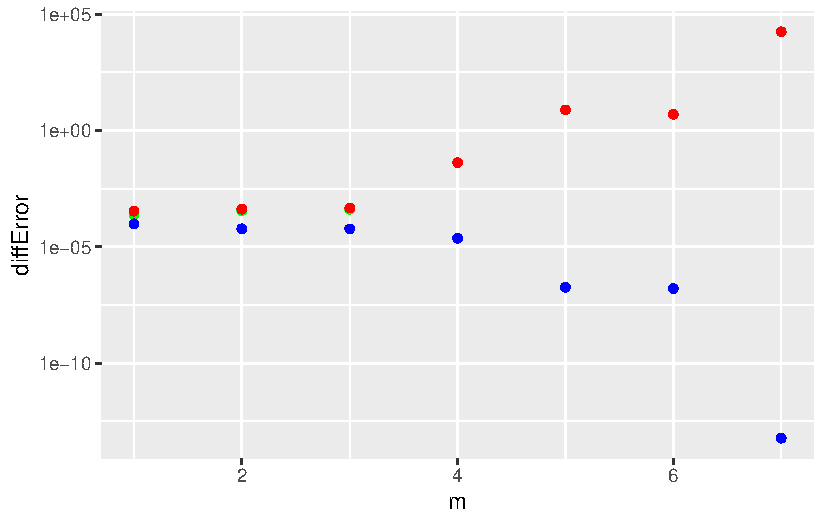
\includegraphics{excercise_doc_files/figure-pdf/unnamed-chunk-3-1.pdf}

}

\end{figure}

\begin{Shaded}
\begin{Highlighting}[]
\FunctionTok{head}\NormalTok{(MSE\_poly,}\DecValTok{7}\NormalTok{)}
\end{Highlighting}
\end{Shaded}

\begin{verbatim}
  m     errTrain      errTest i    diffError logerrTest logerrTrain
1 1 9.783850e-05 3.363816e-04 1 2.385431e-04  -7.997264   -9.232192
2 2 5.942656e-05 4.129855e-04 2 3.535590e-04  -7.792098   -9.730769
3 3 5.884494e-05 4.641982e-04 3 4.053533e-04  -7.675199   -9.740605
4 4 2.318943e-05 4.177533e-02 4 4.175214e-02  -3.175449  -10.671814
5 5 1.818859e-07 7.715585e+00 5 7.715585e+00   2.043242  -15.519886
6 6 1.605274e-07 4.971764e+00 6 4.971764e+00   1.603775  -15.644801
7 7 5.927753e-14 1.756514e+04 7 1.756514e+04   9.773672  -30.456546
\end{verbatim}

\hypertarget{checkpoint-5-b-training--and-test-errors}{%
\subsection{Checkpoint 5: b Training- and test
errors}\label{checkpoint-5-b-training--and-test-errors}}

\begin{enumerate}
\def\labelenumi{(\alph{enumi})}
\item
  Explain the difference between a training- and a test data. Also
  explain the difference between training- and test error.

  The training data is used for training the models for predicting a
  certain outcome. The test data is used to test the trained model, to
  evaluate how well the trained model are predicting. The tools for
  evaluate the models performance is based on training and testing
  error. The training error are the error from the devolped model on the
  trained data point, where it is the same for testing, just focusing on
  the testing data points.
\item
  Argue why we typically are interested in good model performance in
  terms of low test error rather than in terms of low training error.

  We like to prioritize low error test results because the fitted model
  true evaluation depends how it fit with the validation points from
  test data set.
\end{enumerate}

\hypertarget{checkpoint-6-b-do-section-2.4-conceptual-exercise-3.-in-isl-isl-page-53.}{%
\subsection{Checkpoint 6: b Do section 2.4 conceptual exercise 3. in ISL
(ISL page
53).}\label{checkpoint-6-b-do-section-2.4-conceptual-exercise-3.-in-isl-isl-page-53.}}

\begin{enumerate}
\def\labelenumi{\arabic{enumi}.}
\setcounter{enumi}{2}
\tightlist
\item
  We now revisit the bias-variance decomposition.
\end{enumerate}

\begin{enumerate}
\def\labelenumi{(\alph{enumi})}
\tightlist
\item
  Provide a sketch of typical (squared) bias, variance, training error,
  test error, and Bayes (or irreducible) error curves, on a single plot,
  as we go from less flexible statistical learning methods towards more
  flexible approaches. The x-axis should represent the amount of
  flexibility in the method, and the y-axis should represent the values
  for each curve. There should be five curves. Make sure to label each
  one.
\end{enumerate}

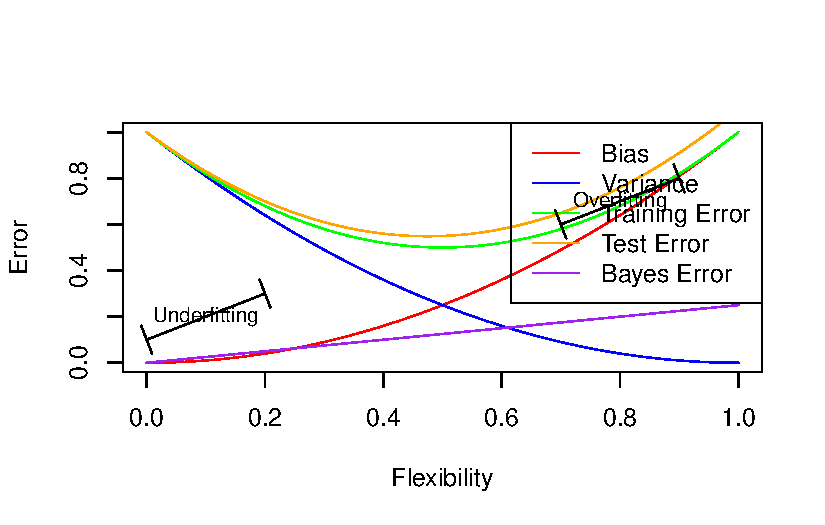
\includegraphics{excercise_doc_files/figure-pdf/unnamed-chunk-4-1.pdf}

\textbf{(b) Explain why each of the five curves has the shape displayed
in part (a).}

\begin{verbatim}
As training error decreases because of better fitting, however overfitting is introduced and causes increase in test error. Bias decrease in training data with the high complexity. However, the trade off is that variance are increasing. So we want to chose the flexibility point were bias and variance in combination are lowest.
\end{verbatim}

\hypertarget{checkpoint-7}{%
\subsection{Checkpoint 7:}\label{checkpoint-7}}

Explain, in your own words, what a training set is, a validation set is,
and a test set is? Why is this partition of data needed? Explain how
k-fold cross validation is implemented. Explain how leave-one-out (LOO)
cross validation is implemented. What are the advantages and
disadvantages of k-fold cross validation relative to the validation set
approach and the LOO cross validation approach?

\begin{verbatim}
Training set is data that is used for training the prediction model, where validation is used for evaluated how well the model predicts the outcome in interest.
\end{verbatim}

\hypertarget{checkpoint-8}{%
\subsection{Checkpoint 8:}\label{checkpoint-8}}

R users: By using the functions createDataPartition and createFolds we
can create random partitions of data.

• Look at the help text for these functions and use a bit of time to
familiarize yourself with the functions.

\begin{enumerate}
\def\labelenumi{(\alph{enumi})}
\tightlist
\item
  Run the command c = createDataPartition(y = 1:20, p = 0.8) and explain
  what the function does. Also describe the content of the variable c.
\end{enumerate}

\emph{It creates a list of numbers (series) of partition from 1 - 20}

\begin{enumerate}
\def\labelenumi{(\alph{enumi})}
\setcounter{enumi}{1}
\tightlist
\item
  Run the command c = createFolds(y = 1:20, k = 10, returnTrain = TRUE)
  and explain what the function does. Also explain the content of the
  variable c.
\end{enumerate}

\emph{CreateFold split up the data in k groups. Here c are devided into
10 k-folds with 20 vector outcomes.}

\begin{enumerate}
\def\labelenumi{(\alph{enumi})}
\setcounter{enumi}{2}
\tightlist
\item
  Explain why it is generally recommended to run e.g.~the command
  set.seed(0) before creating the random partitions.
\end{enumerate}

\emph{To set up the seed before deviding the dataset and doing the
analysis, hence obtain reproduceability.}

\hypertarget{check-point-9}{%
\subsection{Check point 9}\label{check-point-9}}

Linear regression - body density data - cross validation In this
checkpoint you will analyse the body density data using linear
regression (with polynomial regressors), and the goal is to build a
linear regression model to predict body density from chest circumference
measurements. You will use k-fold cross validation to evaluate model
performance for different polynomial order.

• Open the script main1b.m and review it to understand the different
steps in the script. Some of the code needed to answer this checkpoint
is already provided in the script, but you also need to do a bit of
coding yourself. Use the script main1b.m / main1b.R and your code to
answer the following:

\begin{enumerate}
\def\labelenumi{(\alph{enumi})}
\tightlist
\item
  Load the data set bodyMeasurementsSingleCV.txt. Describe the data,
  what is the size of the data set? how many observations and features?
\end{enumerate}

\emph{252 obs and 2 features}

\begin{enumerate}
\def\labelenumi{(\alph{enumi})}
\setcounter{enumi}{1}
\tightlist
\item
  Identify the part of the script where the random partition is
  performed. How many folds are used in the k-fold cross validation?
\end{enumerate}

\emph{10 k-folds}

\begin{enumerate}
\def\labelenumi{(\alph{enumi})}
\setcounter{enumi}{2}
\tightlist
\item
  The script contains two for-loops (one nested within the other).
  Explain, in your own words, how the analysis is performed/structured
  in the script.
\end{enumerate}

\emph{The fist part of the loop is splitting the training data and this
will be done K times (10 in this case). Each data set will be included
another loop with conducting training a linear model with flexibility of
order m ( up till 7 in this case). Each model will tested on each test
data set and errors estimates from train and test evaluation will be
extracted.}

\begin{enumerate}
\def\labelenumi{(\alph{enumi})}
\setcounter{enumi}{3}
\tightlist
\item
  Run the script. Look at the plot of training and test error
  (cross-validation error) (ordinate) vs.~polynomial order (abscissa)
  (both error curves in same plot). Include the plot in your report and
  describe/discuss it. Are the curves as expected? do you observe severe
  overfitting (compare with your result from Checkpoint 4)? if not, try
  to explain why not (Hint: look at the number of training observations
  and model flexibility). For which polynomial order do you observe the
  lowest test error?
\end{enumerate}

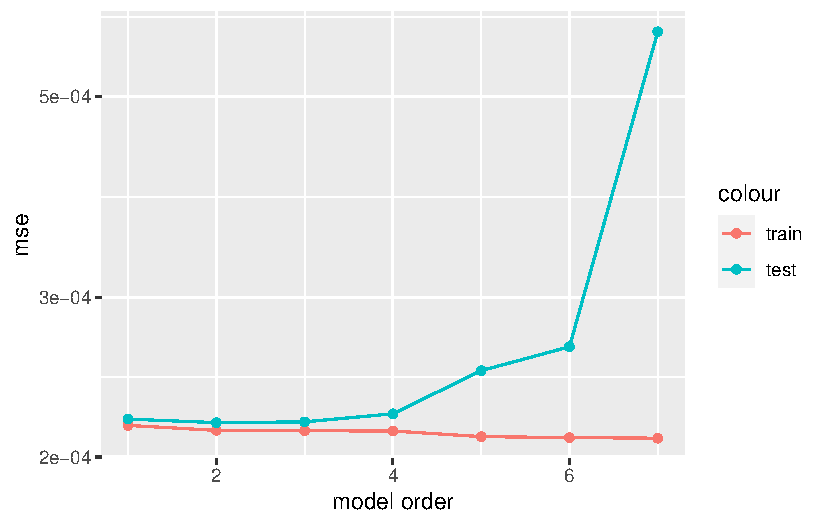
\includegraphics{excercise_doc_files/figure-pdf/unnamed-chunk-5-1.pdf}

\emph{We do not observe the same severity as the earlier models. The
overfitting seem first to be slightly introduced after 5 orders in
polynomial. Again the best model would be using 2 orders in polynomial
as this has the lowest value in MSEtest. The improvement of the model is
expected as we are using more data for training dataset (90\%) and we
are including cross-validation.}

\hypertarget{excercise-day-2}{%
\section{Excercise Day 2}\label{excercise-day-2}}

\hypertarget{logistic-regression}{%
\section{Logistic Regression}\label{logistic-regression}}

\hypertarget{checkpoint-10-the-logistic-regression-model-suppose-that-your-input-data-xi-has-a-single-predictor-xi1-and-suppose-that-the-logistic-regression-model-has-parameters-ux3b20-1-and-ux3b21-1.}{%
\subsection{Checkpoint 10: The logistic regression model Suppose that
your input data xi has a single predictor xi1, and suppose that the
logistic regression model has parameters β0 = 1 and β1 =
1.}\label{checkpoint-10-the-logistic-regression-model-suppose-that-your-input-data-xi-has-a-single-predictor-xi1-and-suppose-that-the-logistic-regression-model-has-parameters-ux3b20-1-and-ux3b21-1.}}

\begin{enumerate}
\def\labelenumi{(\alph{enumi})}
\tightlist
\item
  Make a drawing/plot with curves of i) the posterior probability of
  class 0 P (y = 0\textbar xi) as a function of xi1 and ii) the
  posterior probability of class 1 P (y = 1\textbar xi) as a function of
  xi1, with xi1 ranging from -6 to 6. Remember to label each of the
  curves, to label axes in your drawing, and also remember to put tick
  labeling (numeric) on the axes.
\end{enumerate}

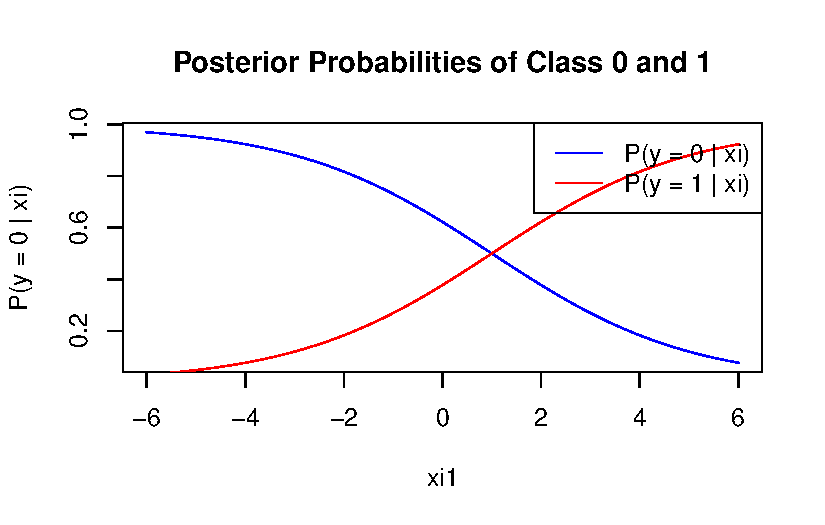
\includegraphics{excercise_doc_files/figure-pdf/unnamed-chunk-6-1.pdf}

\begin{enumerate}
\def\labelenumi{(\alph{enumi})}
\setcounter{enumi}{1}
\tightlist
\item
  Explain how you can classify a given input xi by using the posterior
  probabilities, and indicate the decision boundary/threshold on your
  drawing/plot above.
\end{enumerate}

\emph{Based on xi will the classification be 0 from -6 to 1 because the
have the highest probability wihch is \textgreater{} 0.5. Afterwards,
beyond xi \textgreater{} 1 the probability for y=1 is \textgreater0.5,
and hence will classify to category 1.}

\begin{enumerate}
\def\labelenumi{(\alph{enumi})}
\setcounter{enumi}{2}
\tightlist
\item
  Make another drawing/plot with the log-odds ratio as a function of
  xi1.
\end{enumerate}

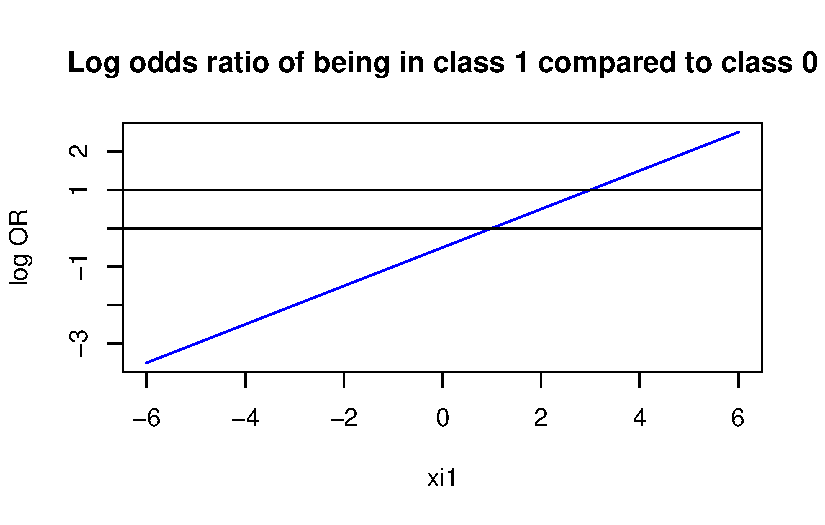
\includegraphics{excercise_doc_files/figure-pdf/unnamed-chunk-7-1.pdf}

\begin{enumerate}
\def\labelenumi{(\alph{enumi})}
\setcounter{enumi}{3}
\tightlist
\item
  Explain how you can classify a given input xi by using the log-odds
  ratio, and indicate the decision boundary/threshold on your
  drawing/plot above.
\end{enumerate}

\emph{When OR are \textgreater1, the probability for being in class 1 is
higher than the probability for being in class 0. Like the first plot
the threshold can be found at xi = 1.}

\begin{enumerate}
\def\labelenumi{(\alph{enumi})}
\setcounter{enumi}{4}
\tightlist
\item
  Suppose that we have three test samples For each of these three
  samples, compute P (y = 1\textbar xi) and compute the predicted the
  class label.
\end{enumerate}

{[}Three
samples{]}here::here(``doc/pics/Screenshot\%202023-01-11\%20at\%2008.30.51.png''))

\begin{Shaded}
\begin{Highlighting}[]
\NormalTok{log\_funk }\OtherTok{\textless{}{-}} \ControlFlowTok{function}\NormalTok{(x) \{}
\NormalTok{post\_prob\_1 }\OtherTok{\textless{}{-}} \FunctionTok{exp}\NormalTok{(}\DecValTok{1}\SpecialCharTok{+}\DecValTok{1}\SpecialCharTok{*}\NormalTok{x)}
\NormalTok{post\_prob\_0 }\OtherTok{\textless{}{-}} \DecValTok{1}\SpecialCharTok{+}\NormalTok{post\_prob\_1}
\NormalTok{Y\_Ix }\OtherTok{\textless{}{-}}\NormalTok{ post\_prob\_1}\SpecialCharTok{/}\NormalTok{post\_prob\_0}

\FunctionTok{return}\NormalTok{(Y\_Ix)}
\NormalTok{\}}
\end{Highlighting}
\end{Shaded}

\begin{Shaded}
\begin{Highlighting}[]
\NormalTok{p\_v }\OtherTok{\textless{}{-}} \FunctionTok{c}\NormalTok{(}\SpecialCharTok{{-}}\DecValTok{2}\NormalTok{,}\DecValTok{0}\NormalTok{,}\DecValTok{2}\NormalTok{)}

\ControlFlowTok{for}\NormalTok{ (i }\ControlFlowTok{in}\NormalTok{ p\_v) \{}
\NormalTok{  y\_val }\OtherTok{\textless{}{-}} \FunctionTok{log\_funk}\NormalTok{(i)}
  \FunctionTok{print}\NormalTok{(y\_val)}
\NormalTok{\}}
\end{Highlighting}
\end{Shaded}

\begin{verbatim}
[1] 0.2689414
[1] 0.7310586
[1] 0.9525741
\end{verbatim}

\hypertarget{checkpoint-11-logistic-regression---csf-biomarker-data}{%
\subsection{Checkpoint 11: Logistic regression - CSF biomarker
data}\label{checkpoint-11-logistic-regression---csf-biomarker-data}}

In this checkpoint you will analyse the CSF biomarker data using
logistic regression. The goal of the analysis is to build a logistic
regression model to predict group membership (control/impaired) from a
single CSF feature tau. • Open the script main2a.m / main2a.R and review
it to understand the different steps in the script.

\begin{Shaded}
\begin{Highlighting}[]
\FunctionTok{source}\NormalTok{(here}\SpecialCharTok{::}\FunctionTok{here}\NormalTok{(}\StringTok{"R/day\_2\_code/main2a.R"}\NormalTok{))}
\end{Highlighting}
\end{Shaded}

\begin{figure}[H]

{\centering 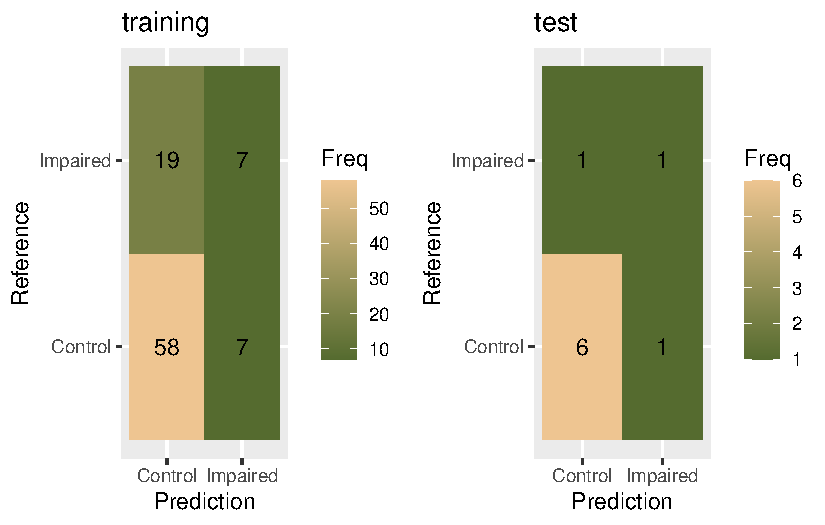
\includegraphics{excercise_doc_files/figure-pdf/unnamed-chunk-10-1.pdf}

}

\end{figure}

\begin{enumerate}
\def\labelenumi{(\alph{enumi})}
\tightlist
\item
  Run the first code section \%\% Import data etc.. What is the size of
  the data set? How many features and observations? Describe the
  response variable y, what type of variable is it and what is its
  content? How many subjects are there in each group?
\end{enumerate}

\emph{100 obs and 131 features}

\begin{verbatim}

 Control Impaired 
      72       28 
\end{verbatim}

\begin{enumerate}
\def\labelenumi{(\alph{enumi})}
\setcounter{enumi}{1}
\tightlist
\item
  Explain how data is divided into a training set and a test set, and
  explain the meaning of stratification. Run the second code section
  \%\% Divide into training and test sets. Compute the class proportions
  in the training set and in the test set and report these, and verify
  that class proportions are preserved after the data partitioning.
\end{enumerate}

\emph{By using the code createDataPartition, and specify that Y should
be account for the two outcomes, and define that 90\% of data goes to
training.}

\begin{enumerate}
\def\labelenumi{(\alph{enumi})}
\setcounter{enumi}{2}
\tightlist
\item
  Run the code section \%\% Train model, predict, and plot model.
  Describe the variable catInfo and its content. Describe the model
  outputs yhatTrainProb and yhatTestProb, what does these represent?
  Describe the variables yhatTrain and yhatTest, what do these
  represent? Include the plot of model output vs.~input, describe the
  plot, and explain how classification can be performed based on this
  plot.
\end{enumerate}

\emph{catInfo is the variable including the labels of the group response
(impaired/control). yhatTrainProb is the predicted groups in training
data set based on the trained model, and yhatTestProb is the predicted
groups in the testing data set based on the trained model (validation of
the model). yhatTrain and yhatTest are rounded the probabilities of
yhatTrainProb and yhatTestProb to a single digit, a 0 or 1 to be
classified as imparied or control. Approximately, if the tau value was
above 6.5 you had a higher probability for being in imparired compared
to control}

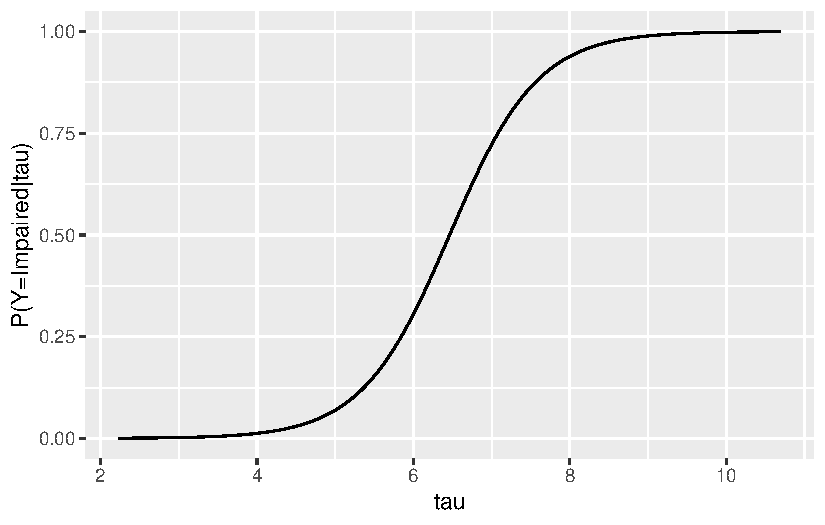
\includegraphics{excercise_doc_files/figure-pdf/unnamed-chunk-12-1.pdf}

\begin{enumerate}
\def\labelenumi{(\alph{enumi})}
\setcounter{enumi}{3}
\tightlist
\item
  In the third code section, the model predictions are converted to
  categorical data to be used as input to the confusionchart (Matlab)
  confusionMatrix (R) function for plotting the confusion matrix. Look
  at the help text for this function and use a bit of time to
  familiarize yourself with the function. Run the forth code section
  \%\% Plot confusion matrix, include the plot in your report, and
  describe/discuss it. Based on the numbers in the confusion matrix,
  compute and report the following performance metrics for the test set:
  classification accuracy, error rate, true positive rate, true negative
  rate, false positive rate, false negative rate, sensitivity, and
  specificity.
\end{enumerate}

\emph{When plotting the confusion matrix, we observe the the abbility of
the trained model to predict outcome, hence its performance compared
with th actual observation in both the traing and testing dataset,
retrospectively}

\emph{Based on visual observing the plots and estimates of
classification accuracy, error rate, true positive rate, true negative
rate, false positive rate, false negative rate, sensitivity, and
specificity, the models performance are quite poor especially to detect
observation with impaired status. This are also reflected by the low
sensitivity and true positive predictive value. On the other hand the
model performs well to detect, observations in control group, which are
the reason the error rate accuracy does not have too bad performance.}

\begin{Shaded}
\begin{Highlighting}[]
\CommentTok{\#|eecho: false}

\FunctionTok{grid.arrange}\NormalTok{(cm\_train\_plot, cm\_test\_plot, }\AttributeTok{ncol =} \DecValTok{2}\NormalTok{)}
\end{Highlighting}
\end{Shaded}

\begin{figure}[H]

{\centering 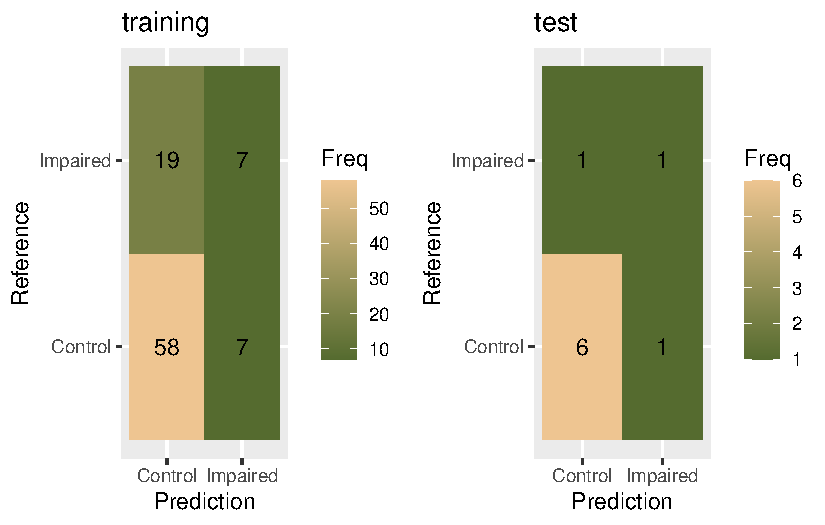
\includegraphics{excercise_doc_files/figure-pdf/unnamed-chunk-13-1.pdf}

}

\end{figure}

\begin{Shaded}
\begin{Highlighting}[]
\CommentTok{\#Training data}
\NormalTok{report\_prec\_train}
\end{Highlighting}
\end{Shaded}

\begin{verbatim}
     true_pr false_pr   true_nr  false_nr      sens      spec
[1,]     0.5      0.5 0.7532468 0.2467532 0.2692308 0.8923077
\end{verbatim}

\begin{Shaded}
\begin{Highlighting}[]
\NormalTok{accTrain }\CommentTok{\#accuracy}
\end{Highlighting}
\end{Shaded}

\begin{verbatim}
[1] 0.7142857
\end{verbatim}

\begin{Shaded}
\begin{Highlighting}[]
\NormalTok{errTrain }\CommentTok{\#error rate}
\end{Highlighting}
\end{Shaded}

\begin{verbatim}
[1] 0.2857143
\end{verbatim}

\begin{Shaded}
\begin{Highlighting}[]
\CommentTok{\# Testing data}
\NormalTok{report\_prec\_test}
\end{Highlighting}
\end{Shaded}

\begin{verbatim}
     true_pr false_pr   true_nr  false_nr sens      spec
[1,]     0.5      0.5 0.8571429 0.1428571  0.5 0.8571429
\end{verbatim}

\begin{Shaded}
\begin{Highlighting}[]
\NormalTok{accTest }\CommentTok{\#accuracy}
\end{Highlighting}
\end{Shaded}

\begin{verbatim}
[1] 0.7777778
\end{verbatim}

\begin{Shaded}
\begin{Highlighting}[]
\NormalTok{errTest }\CommentTok{\#error rate}
\end{Highlighting}
\end{Shaded}

\begin{verbatim}
[1] 0.2222222
\end{verbatim}

\begin{enumerate}
\def\labelenumi{(\alph{enumi})}
\setcounter{enumi}{4}
\tightlist
\item
  You will now do almost the same analysis, but you will now use 10-fold
  cross-validation for model evaluation. Open the script main2b.m /
  main2b.R and review it to understand the different steps in the
  script. Run the script. Include the plot of the confusion matrices for
  the trainingand test/validation data in you report and
  describe/discuss it. Also explain how the confusion matrices are
  computed across the cross-validation iterations. Based on the numbers
  in the confusion matrix, compute and report the following performance
  metrics for the test set: classification accuracy, error rate, true
  positive rate, true negative rate, false positive rate, false negative
  rate, sensitivity, and specificity.
\end{enumerate}

\emph{When using the cross-validation, we are having a loop with K (10
in this case) different training and testing data set. Based on the
loop, we estimate the average values from the loop estimates into the
confusion matrix. The new developed model with cross-validation have
higher accuracy and lower error rate in training data, compare to the
simpler model from main2a, however the testing data are more imprecise
compared to earlier model. Again, the model performs well, to find true
control and have high specificity. The sensitivity was improved in the
training, but performed horrible in the testing data set, with no
sensitivity at all to capture impaired}

\begin{Shaded}
\begin{Highlighting}[]
\CommentTok{\#|echo: false}
\FunctionTok{grid.arrange}\NormalTok{(cm\_train\_plot,cm\_test\_plot, }\AttributeTok{ncol =} \DecValTok{2}\NormalTok{)}
\end{Highlighting}
\end{Shaded}

\begin{figure}[H]

{\centering 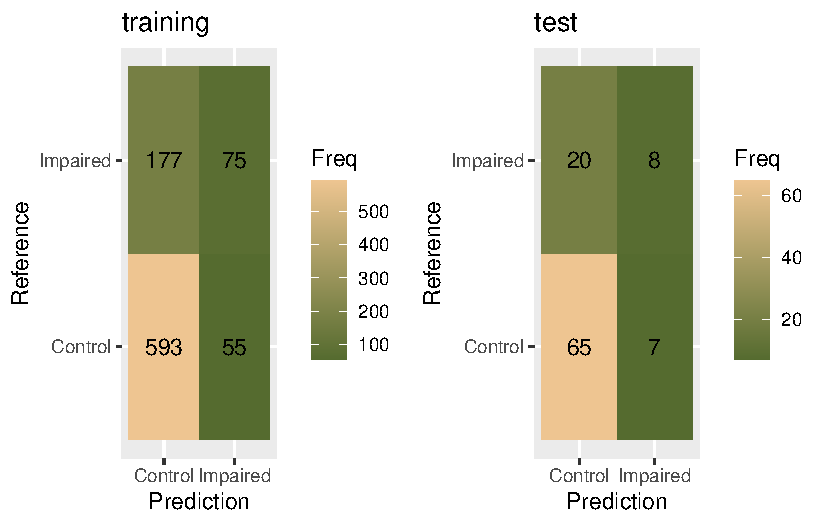
\includegraphics{excercise_doc_files/figure-pdf/unnamed-chunk-16-1.pdf}

}

\end{figure}

\begin{Shaded}
\begin{Highlighting}[]
\CommentTok{\#Training data}
\NormalTok{report\_prec\_train}
\end{Highlighting}
\end{Shaded}

\begin{verbatim}
       true_pr  false_pr   true_nr  false_nr sens      spec
[1,] 0.6666667 0.3333333 0.7820513 0.2179487 0.32 0.9384615
\end{verbatim}

\begin{Shaded}
\begin{Highlighting}[]
\NormalTok{accTrain[idx1] }\CommentTok{\#accuracy}
\end{Highlighting}
\end{Shaded}

\begin{verbatim}
[1] 0.7666667
\end{verbatim}

\begin{Shaded}
\begin{Highlighting}[]
\NormalTok{errTrain[idx1] }\CommentTok{\#error rate}
\end{Highlighting}
\end{Shaded}

\begin{verbatim}
[1] 0.2333333
\end{verbatim}

\begin{Shaded}
\begin{Highlighting}[]
\CommentTok{\# Testing data}
\NormalTok{report\_prec\_test}
\end{Highlighting}
\end{Shaded}

\begin{verbatim}
     true_pr false_pr   true_nr  false_nr sens      spec
[1,]       0        1 0.6666667 0.3333333    0 0.8571429
\end{verbatim}

\begin{Shaded}
\begin{Highlighting}[]
\NormalTok{accTest[idx1] }\CommentTok{\#accuracy}
\end{Highlighting}
\end{Shaded}

\begin{verbatim}
[1] 0.6
\end{verbatim}

\begin{Shaded}
\begin{Highlighting}[]
\NormalTok{errTest[idx1] }\CommentTok{\#error rate}
\end{Highlighting}
\end{Shaded}

\begin{verbatim}
[1] 0.4
\end{verbatim}

\hypertarget{checkpoint-12-regularization}{%
\subsection{Checkpoint 12:
Regularization}\label{checkpoint-12-regularization}}

\begin{enumerate}
\def\labelenumi{(\alph{enumi})}
\tightlist
\item
  Explain when and why it may be necessary to use model regularization.
\end{enumerate}

\emph{To constrain the flexibility/complexity of the model and decrease
the MSE. Here our goal is to minimize the error caused by variance and
bias, and in the end improve the robustness of the models ability to
predict, and prevent overfitting}

\begin{enumerate}
\def\labelenumi{(\alph{enumi})}
\setcounter{enumi}{1}
\item
  \begin{enumerate}
  \def\labelenumii{(\arabic{enumii})}
  \tightlist
  \item
    Write down the penalized cost function for linear regression for
    each of the following penalty/shrinkage terms: (i) ridge (ℓ2), (ii)
    lasso (ℓ1).
  \end{enumerate}
\end{enumerate}

\emph{In ridge, the values shrinkage close to zero and MSE decrease
until a certain value. In lasso, some coefficients shrink to zero and
the most important features are left.}

\begin{enumerate}
\def\labelenumi{(\arabic{enumi})}
\setcounter{enumi}{1}
\tightlist
\item
  Explain meaning of the different elements of the expressions in (1).
\end{enumerate}

\emph{The residual sum of sqaure that, sum each obesevation true value
minus their predicted value.}

\hypertarget{checkpoint-13-b-regularization-training--and-test-errors-and-biasvariance-trade-off}{%
\subsection{Checkpoint 13: b Regularization, training- and test errors,
and biasvariance
trade-off}\label{checkpoint-13-b-regularization-training--and-test-errors-and-biasvariance-trade-off}}

\begin{enumerate}
\def\labelenumi{(\alph{enumi})}
\tightlist
\item
  Provide a sketch of how coefficient estimates typically change with
  the strength of the regularization parameter λ for the ridge and the
  lasso penalty, respectively. Describe/discuss the curves and their
  similarities/differences.
\end{enumerate}

\emph{Ridge /} \emph{Lasso}

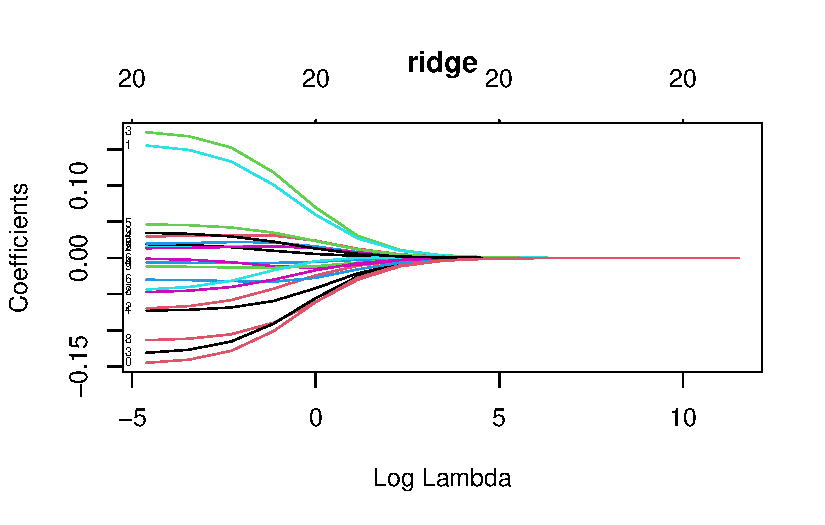
\includegraphics{excercise_doc_files/figure-pdf/unnamed-chunk-18-1.pdf}

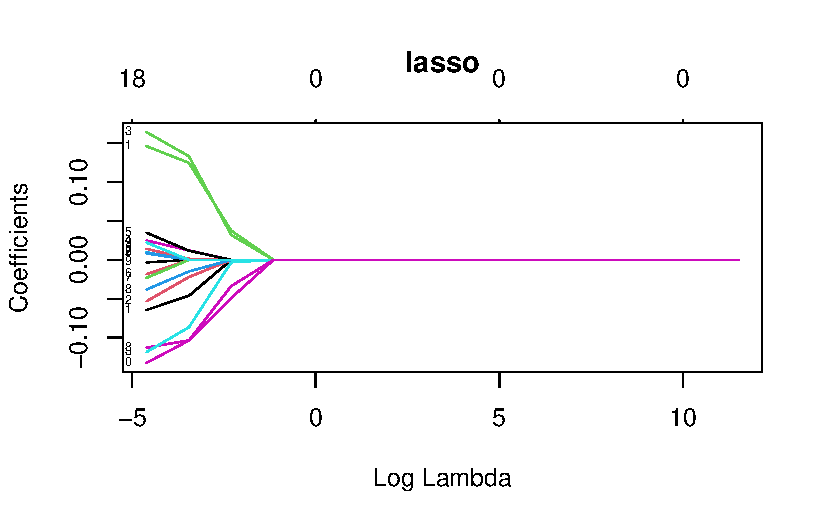
\includegraphics{excercise_doc_files/figure-pdf/unnamed-chunk-18-2.pdf}


\includegraphics{excercise_doc_files/figure-pdf/unnamed-chunk-18-3.pdf}

\emph{Both regularization methods are shrinking values to improve model
performance. In ridge, all coefficients are shrinkage collectively,
where in lasso some coefficients are shrinkage to 0 and some increases
in beta value.}

\begin{enumerate}
\def\labelenumi{(\alph{enumi})}
\tightlist
\item
  Provide a sketch of typical training error and test error on a single
  plot, as a function of the regularization parameter λ. λ should be on
  the x-axis, and the y-axis should represent the values for each curve.
  Make sure to label each one.
\end{enumerate}

\begin{itemize}
\tightlist
\item
\end{itemize}

\hypertarget{read-up-in-isl}{%
\subsection{READ UP IN ISL}\label{read-up-in-isl}}

Ridge /lasso
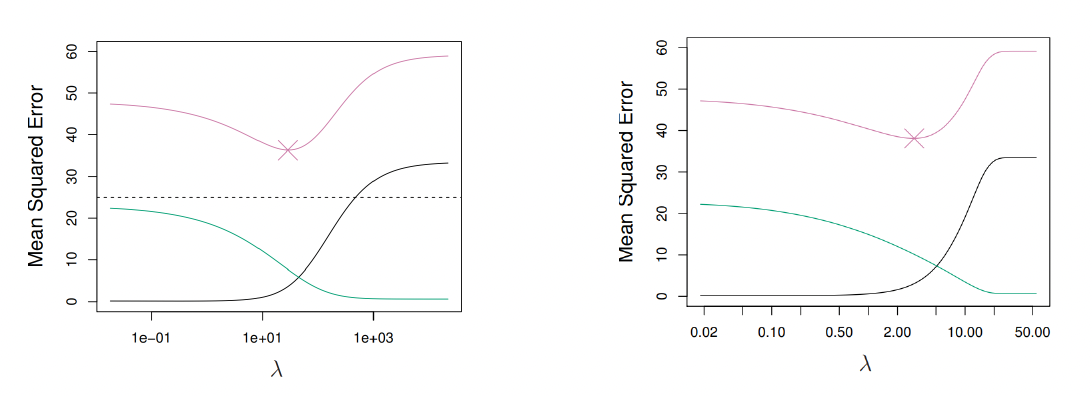
\includegraphics{desktop/r_directory/courses/AU_applied_machine_learning_health_science/doc/pics/Screenshot 2023-01-11 at 11.06.44.png}

\begin{enumerate}
\def\labelenumi{(\alph{enumi})}
\setcounter{enumi}{1}
\tightlist
\item
  Explain why each of the two curves has the shape displayed in (a).
\end{enumerate}

\emph{Squared bias (black), variance(green), test error(purple). Between
the variance and bias there occurs a sweet optimal spot for MSE, where
MSE is lowest. Afterward, the bias increases and the variance
decreases.}

\begin{enumerate}
\def\labelenumi{(\alph{enumi})}
\setcounter{enumi}{2}
\tightlist
\item
  Explain how model complexity changes with λ, and discuss your answer
  in terms of the bias-variance trade-off.
\end{enumerate}

\emph{see above discription}

\begin{enumerate}
\def\labelenumi{(\alph{enumi})}
\setcounter{enumi}{3}
\tightlist
\item
  Explain how the suitable regularization strength is chosen in a
  real-world analysis.
\end{enumerate}

\emph{By using cross-validation, and observe the the model performance
on trainig data and testing data. We want to choose the lambda value
based on the model }

\hypertarget{checkpoint-14-linear-regression---body-density-data---ridge-regularization}{%
\subsection{Checkpoint 14: Linear regression - body density data - ridge
regularization}\label{checkpoint-14-linear-regression---body-density-data---ridge-regularization}}

In this checkpoint you will analyse the body density data using linear
regression, and the goal is to build a ridge regularized linear
regression model to predict body density based on subjects' age, height,
weight, and 10 circumference measurements (13 input features in total).
You will use k-fold cross-validation to evaluate model performance for
different regularization strengths.

• Open the script main3a.m / main3a.R and review it to understand the
different steps in the script.

Use the script and your code to answer the following: (a) Load the data
set bodyMeasurements.txt. Describe the data, what is the size of the
data set? how many observations and features?

\emph{252 obs with 14 features}

\begin{enumerate}
\def\labelenumi{(\alph{enumi})}
\setcounter{enumi}{1}
\tightlist
\item
  Identify the part of the script where the random partition is
  performed. How many folds are used in the k-fold cross-validation?
\end{enumerate}

\emph{Using createKolfold where there are used 10 k-folds}

\begin{enumerate}
\def\labelenumi{(\alph{enumi})}
\setcounter{enumi}{2}
\tightlist
\item
  Identify the part of the script where the range of the regularization
  parameter λ is defined. Which sequence of λ-values is used?
\end{enumerate}

\emph{lambda = 2\^{}seq(5, -15, by = -0.5) spanning form 5 to -15 by
each -0.5}

\begin{enumerate}
\def\labelenumi{(\alph{enumi})}
\setcounter{enumi}{3}
\tightlist
\item
  The script contains two for-loops (one nested within the other).
  Explain, in your own words, how the analysis is performed/structured
  in the script.
\end{enumerate}

\emph{In the first loop, we are defining the training and the testing
data set by each k-folds, then a fitted model with different lambda
values are established using the training set, by the function glm
family gaussian. Then the predicted value for training and testing data
set are done. In the second loop, we define matrices with MSE (as ridge
principals), by the different lambda values.}

\begin{enumerate}
\def\labelenumi{(\alph{enumi})}
\setcounter{enumi}{4}
\tightlist
\item
  Identify the lines where data is being standardized in the script.
  Explain how standardization is done, and why it is generally
  recommended to standardize data when using shrinkage regularization.
\end{enumerate}

\begin{itemize}
\tightlist
\item
\end{itemize}

\begin{enumerate}
\def\labelenumi{(\alph{enumi})}
\setcounter{enumi}{5}
\tightlist
\item
  The fitting function has a parameter alpha. Explain what this
  parameter is?
\end{enumerate}

\begin{itemize}
\tightlist
\item
\end{itemize}

\begin{enumerate}
\def\labelenumi{(\alph{enumi})}
\setcounter{enumi}{6}
\tightlist
\item
  Run the analysis. Plot the training error and the test error as a
  function of the regularization parameter λ. Include the plot in your
  report and describe/discuss it.
\end{enumerate}

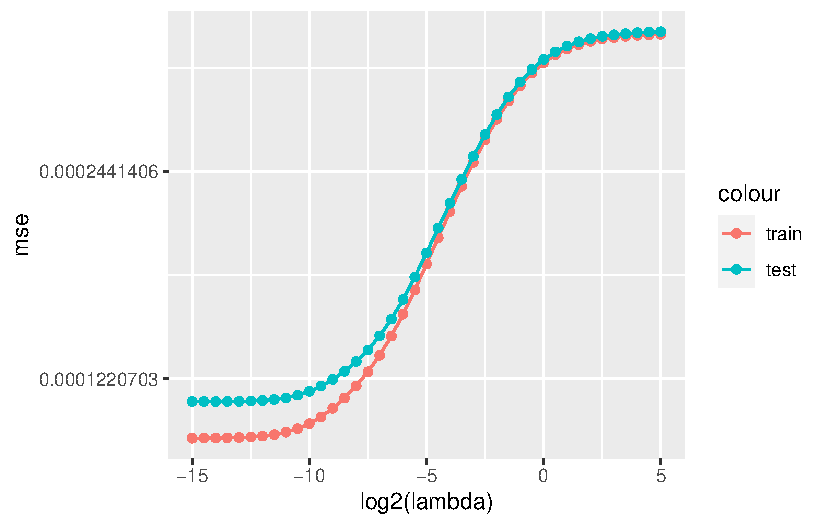
\includegraphics{excercise_doc_files/figure-pdf/unnamed-chunk-20-1.pdf}

\begin{enumerate}
\def\labelenumi{(\alph{enumi})}
\setcounter{enumi}{7}
\tightlist
\item
  How would you choose the ``best'' model? For the selected model report
  the training and test error.
\end{enumerate}

\emph{by visually observing the plot, I would choose the lowest lambda
value plot (-15) because the testing are lowest for this model}

\begin{enumerate}
\def\labelenumi{(\roman{enumi})}
\tightlist
\item
  Look at the β coefficient array. What is the dimensionality of β?
\end{enumerate}

\begin{itemize}
\tightlist
\item
\end{itemize}

\begin{enumerate}
\def\labelenumi{(\alph{enumi})}
\setcounter{enumi}{9}
\tightlist
\item
  Include the plot with coefficient traces as a function of λ in your
  report and describe/discuss it. What happens with coefficients with
  decreased model complexity/ regularization strength? Are any
  coefficients exactly zero?
\end{enumerate}

\emph{As lamba increase the coefficients are shrinkage and the
complexity of the model becomes smaller. Because of this being a ridge
regularization, none of the coefficients are becoming exactly zero, but
just are very small value}

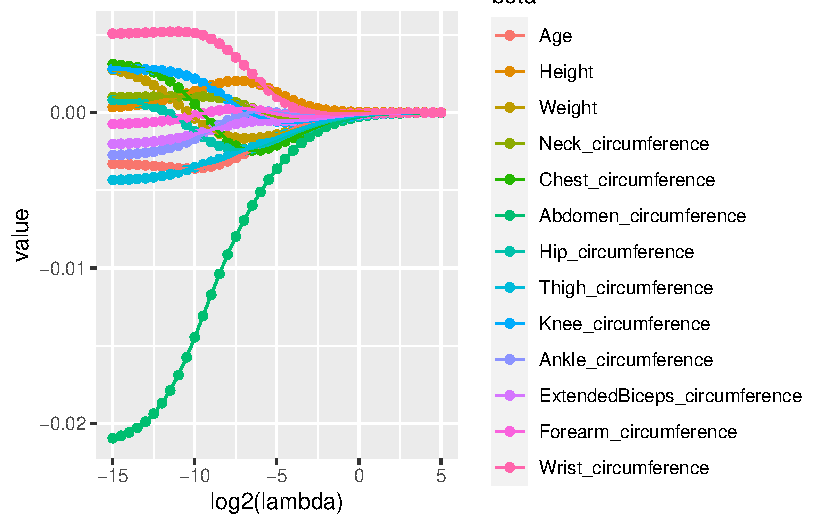
\includegraphics{excercise_doc_files/figure-pdf/unnamed-chunk-21-1.pdf}

\begin{enumerate}
\def\labelenumi{(\alph{enumi})}
\setcounter{enumi}{10}
\tightlist
\item
  Look at the coefficients for your chosen model. Identify the most
  important coefficients to the model.
\end{enumerate}

\emph{The four most important coefficients is abdomen circumference,
wrist circumference, thigh circumference and age}

\hypertarget{checkpoint-15-logistic-regression---csf-biomarker-data---lasso-regularization}{%
\subsection{Checkpoint 15: Logistic regression - CSF biomarker data -
lasso
regularization}\label{checkpoint-15-logistic-regression---csf-biomarker-data---lasso-regularization}}

In this checkpoint you will analyse the CSF biomarker data using
logistic regression with lasso regularization. The goal of the analysis
is to build a logistic regression model to predict group membership
(control/impaired) based on 130 CSF features.

• Open the script main3b.m / main3b.R and review it to understand the
different steps in the script.

Use the script to answer the following:

\begin{enumerate}
\def\labelenumi{(\alph{enumi})}
\tightlist
\item
  Load the data set csfBiomarkers.txt. Describe the data, what is the
  size of the data set? how many observations and features?
\end{enumerate}

\begin{itemize}
\tightlist
\item
\end{itemize}

\begin{enumerate}
\def\labelenumi{(\alph{enumi})}
\setcounter{enumi}{1}
\item
  Identify the part of the script where the random partition is
  performed. How many folds are used in the k-fold cross-validation?
\item
  Identify the part of the script where the range of the regularization
  parameter λ is defined. Which sequence of λ-values is used?
\item
  The script contains two for-loops (one nested within the other).
  Explain, in your own words, how the analysis is performed/structured
  in the script.
\item
  Describe meaning of the fitting function's parameter alpha.
\item
  Run the analysis. Plot the training error and the test error as a
  function of the regularization parameter λ. Include the plot in your
  report and describe/discuss it.
\item
  How would you choose the ``best'' model? For the selected model report
  the training and test error.
\item
  Look at the β coefficient array. What is the dimensionality of β?
\item
  Include the plot with coefficient traces as a function of λ in your
  report and describe/discuss it. What happens with coefficients with
  decreased model complexity/ regularization strength? Are any
  coefficients exactly zero?
\item
  Look at the coefficients for your chosen model. Identify the most
  important coefficients to the model.
\item
  Plot the confusion matrix for your chosen model. Include it in your
  report and describe/discuss it. Based on the numbers in the confusion
  matrix, compute and report the following performance metrics for the
  test set: classification accuracy,error rate, true positive rate, true
  negative rate, false positive rate, false negative rate, sensitivity,
  and specificity.
\end{enumerate}

\hypertarget{support-vector-machines}{%
\section{7 Support vector machines}\label{support-vector-machines}}

\hypertarget{checkpoint-16-bmaximal-margin-classifier}{%
\subsection{Checkpoint 16: bmaximal margin
classifier}\label{checkpoint-16-bmaximal-margin-classifier}}

\begin{enumerate}
\def\labelenumi{(\alph{enumi})}
\tightlist
\item
  Do section 9.7 conceptual exercise 3. in ISL (ISL page 399).
\end{enumerate}

\begin{enumerate}
\def\labelenumi{\arabic{enumi}.}
\setcounter{enumi}{2}
\tightlist
\item
  Here we explore the maximal margin classifier on a toy data set. 9.7
  Exercises 399
\end{enumerate}

\begin{enumerate}
\def\labelenumi{(\alph{enumi})}
\tightlist
\item
  We are given n = 7 observations in p = 2 dimensions. For each
  observation, there is an associated class label. Obs. X1 X2 Y 1 3 4
  Red 2 2 2 Red 3 4 4 Red 4 1 4 Red 5 2 1 Blue 6 4 3 Blue 7 4 1 Blue
  Sketch the observations.
\end{enumerate}

\begin{Shaded}
\begin{Highlighting}[]
\NormalTok{hyper }\OtherTok{\textless{}{-}} \ControlFlowTok{function}\NormalTok{(x1,x2) \{}
\NormalTok{x2\_kor  }\OtherTok{\textless{}{-}} \DecValTok{1} \SpecialCharTok{+} \DecValTok{2}\SpecialCharTok{*}\NormalTok{x1}\DecValTok{{-}3} 
\NormalTok{x1\_kor  }\OtherTok{\textless{}{-}} \DecValTok{1} \SpecialCharTok{+} \DecValTok{3}\SpecialCharTok{*}\NormalTok{x2}\DecValTok{{-}2}
\NormalTok{    kor }\OtherTok{\textless{}{-}} \FunctionTok{cbind}\NormalTok{(x1\_kor,x2\_kor)}
    \FunctionTok{return}\NormalTok{(kor)\}}

\FunctionTok{hyper}\NormalTok{(}\DecValTok{3}\NormalTok{,}\DecValTok{1}\NormalTok{)}
\end{Highlighting}
\end{Shaded}

\begin{verbatim}
     x1_kor x2_kor
[1,]      2      4
\end{verbatim}

\begin{Shaded}
\begin{Highlighting}[]
\NormalTok{df }\OtherTok{\textless{}{-}} \FunctionTok{data.frame}\NormalTok{(}\AttributeTok{obs =} \FunctionTok{c}\NormalTok{(}\DecValTok{1}\SpecialCharTok{:}\DecValTok{7}\NormalTok{),}
                 \AttributeTok{x1 =} \FunctionTok{c}\NormalTok{(}\DecValTok{3}\NormalTok{,}\DecValTok{2}\NormalTok{,}\DecValTok{4}\NormalTok{,}\DecValTok{1}\NormalTok{,}\DecValTok{2}\NormalTok{,}\DecValTok{4}\NormalTok{,}\DecValTok{4}\NormalTok{),}
                 \AttributeTok{x2 =} \FunctionTok{c}\NormalTok{(}\DecValTok{3}\NormalTok{,}\DecValTok{2}\NormalTok{,}\DecValTok{4}\NormalTok{,}\DecValTok{4}\NormalTok{,}\DecValTok{1}\NormalTok{,}\DecValTok{3}\NormalTok{,}\DecValTok{1}\NormalTok{),}
                 \AttributeTok{y =} \FunctionTok{c}\NormalTok{(}\StringTok{"red"}\NormalTok{,}\StringTok{"red"}\NormalTok{,}\StringTok{"red"}\NormalTok{,}\StringTok{"red"}\NormalTok{, }\StringTok{"blue"}\NormalTok{, }\StringTok{"blue"}\NormalTok{, }\StringTok{"blue"}\NormalTok{))}
\end{Highlighting}
\end{Shaded}

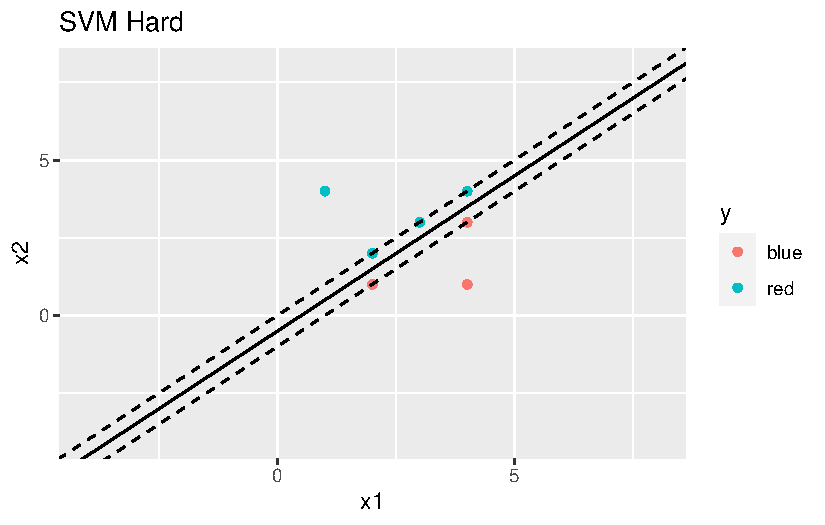
\includegraphics{excercise_doc_files/figure-pdf/unnamed-chunk-24-1.pdf}

\begin{enumerate}
\def\labelenumi{(\alph{enumi})}
\setcounter{enumi}{1}
\item
  Sketch the optimal separating hyperplane, and provide the equation for
  this hyperplane (of the form (9.1)).
\item
  Describe the classification rule for the maximal margin classifier. It
  should be something along the lines of ``Classify to Red if β0 +β1X1
  +β2X2 \textgreater{} 0, and classify to Blue otherwise.'' Provide the
  values for β0, β1, and β2.
\end{enumerate}

\emph{The maximize the suporting vector on both sides of the hyperplane
to the nearst point. This, will be defined as the maximized margin on
both sides, \textgreater0 and \textgreater0 , respectively.}

\begin{enumerate}
\def\labelenumi{(\alph{enumi})}
\setcounter{enumi}{3}
\tightlist
\item
  On your sketch, indicate the margin for the maximal margin hyperplane.
\end{enumerate}

\begin{Shaded}
\begin{Highlighting}[]
\NormalTok{svm\_soft\_plot }\OtherTok{\textless{}{-}}\NormalTok{ df }\SpecialCharTok{\%\textgreater{}\%} 
    \FunctionTok{ggplot}\NormalTok{(}\FunctionTok{aes}\NormalTok{(}\AttributeTok{x =}\NormalTok{ x1, }\AttributeTok{y =}\NormalTok{ x2, }\AttributeTok{group =}\NormalTok{ y), }\AttributeTok{color =} \FunctionTok{factor}\NormalTok{(y))}\SpecialCharTok{+}
    \FunctionTok{geom\_point}\NormalTok{(}\FunctionTok{aes}\NormalTok{(}\AttributeTok{col=}\NormalTok{y))}\SpecialCharTok{+}
    \FunctionTok{geom\_abline}\NormalTok{(}\AttributeTok{slope =} \DecValTok{1}\NormalTok{, }\AttributeTok{intercept =} \SpecialCharTok{{-}}\FloatTok{0.5}\NormalTok{)}\SpecialCharTok{+}
    \FunctionTok{geom\_abline}\NormalTok{(}\AttributeTok{slope =} \DecValTok{1}\NormalTok{, }\AttributeTok{intercept =} \DecValTok{3}\NormalTok{, }\AttributeTok{lty =} \DecValTok{2}\NormalTok{) }\SpecialCharTok{+}
    \FunctionTok{geom\_abline}\NormalTok{(}\AttributeTok{slope =} \DecValTok{1}\NormalTok{, }\AttributeTok{intercept =} \SpecialCharTok{{-}}\FloatTok{3.5}\NormalTok{, }\AttributeTok{lty =} \DecValTok{2}\NormalTok{)}\SpecialCharTok{+}
    \FunctionTok{labs}\NormalTok{(}\AttributeTok{title=}\StringTok{"SVM soft"}\NormalTok{) }\SpecialCharTok{+}
    \FunctionTok{ylim}\NormalTok{(}\FunctionTok{c}\NormalTok{(}\SpecialCharTok{{-}}\DecValTok{4}\NormalTok{,}\DecValTok{8}\NormalTok{))}\SpecialCharTok{+}
    \FunctionTok{xlim}\NormalTok{(}\FunctionTok{c}\NormalTok{(}\SpecialCharTok{{-}}\DecValTok{4}\NormalTok{,}\DecValTok{8}\NormalTok{))}
\FunctionTok{plot}\NormalTok{(svm\_soft\_plot)}
\end{Highlighting}
\end{Shaded}

\begin{figure}[H]

{\centering 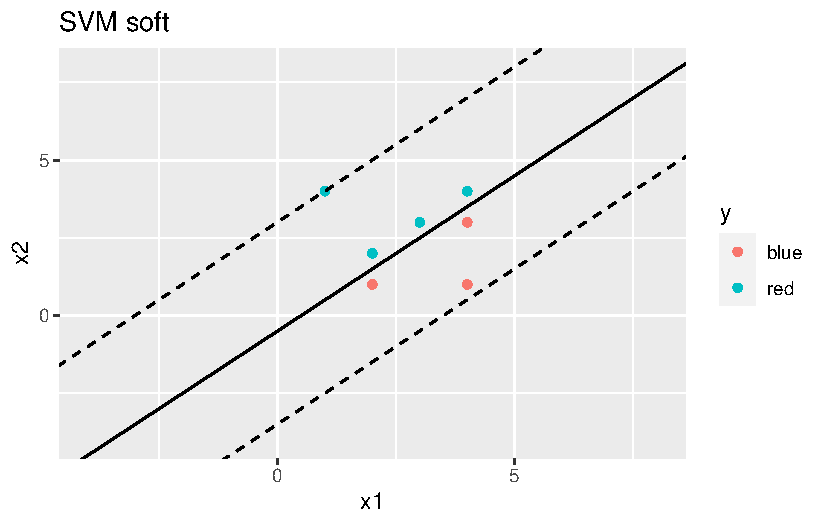
\includegraphics{excercise_doc_files/figure-pdf/unnamed-chunk-25-1.pdf}

}

\end{figure}

\begin{enumerate}
\def\labelenumi{(\alph{enumi})}
\setcounter{enumi}{4}
\item
  Indicate the support vectors for the maximal margin classifier.
\item
  Argue that a slight movement of the seventh observation would not
  affect the maximal margin hyperplane.
\end{enumerate}

\emph{Because the 7th measurement is outside the suporting vector and,
thus are not included in the maximal margins}

\begin{enumerate}
\def\labelenumi{(\alph{enumi})}
\setcounter{enumi}{6}
\item
  Sketch a hyperplane that is not the optimal separating hyperplane, and
  provide the equation for this hyperplane.
\item
  Draw an additional observation on the plot so that the two classes are
  no longer separable by a hyperplane.
\end{enumerate}

\hypertarget{checkpoint-17-support-vector-classifier-aka.-soft-margin-svm}{%
\subsection{Checkpoint 17: Support vector classifier (aka. soft margin
SVM)}\label{checkpoint-17-support-vector-classifier-aka.-soft-margin-svm}}

\begin{enumerate}
\def\labelenumi{(\alph{enumi})}
\tightlist
\item
  Discuss the difference between the maximal margin classifier (hard
  margin SVM) and the support vector classifier (soft margin SVM).
\end{enumerate}

\emph{We define the margin, and find which hyperplane where margin is
maximized. In hard margin we want to maximise the parrallel lines of the
hyperplane (margin) to the nearest support vectors points on both sides
of the hyperplane. In soft margin the support vectors are allowed
constrains, and extend the margins by the value C, and increase the
robustness of the model.}

\begin{enumerate}
\def\labelenumi{(\alph{enumi})}
\setcounter{enumi}{1}
\tightlist
\item
  Describe why it may be necessary or beneficial to use the soft margin
  SVM instead of a hard margin SVM.
\end{enumerate}

\emph{to make a more flexible and robust model, including more vector
points. If the distribution of data does have a clear distiction the
model decision boarder can be unflexible, when using hard margin.
Therefore, sometimes we want to make a more flexible decision boarder}

\begin{enumerate}
\def\labelenumi{(\alph{enumi})}
\setcounter{enumi}{2}
\tightlist
\item
  What are slack variables ϵ?
\end{enumerate}

\emph{The distance to the corresponding canonical hyperplane. How much
slack variables with allow to individual points.}

\begin{enumerate}
\def\labelenumi{(\alph{enumi})}
\setcounter{enumi}{3}
\tightlist
\item
  Discuss the meaning of the regularization parameter C.
\end{enumerate}

\emph{C is to control how much we want to extend our margin variation in
canonical hyperplane. When we increase C we tend to include more
supporting vectors.}

\begin{enumerate}
\def\labelenumi{(\alph{enumi})}
\setcounter{enumi}{4}
\tightlist
\item
  On your sketch from the previous checkpoint, draw an example of a soft
  margin.
\end{enumerate}

\begin{Shaded}
\begin{Highlighting}[]
\NormalTok{svm\_soft\_plot }\OtherTok{\textless{}{-}}\NormalTok{ df }\SpecialCharTok{\%\textgreater{}\%} 
    \FunctionTok{ggplot}\NormalTok{(}\FunctionTok{aes}\NormalTok{(}\AttributeTok{x =}\NormalTok{ x1, }\AttributeTok{y =}\NormalTok{ x2, }\AttributeTok{group =}\NormalTok{ y), }\AttributeTok{color =} \FunctionTok{factor}\NormalTok{(y))}\SpecialCharTok{+}
    \FunctionTok{geom\_point}\NormalTok{(}\FunctionTok{aes}\NormalTok{(}\AttributeTok{col=}\NormalTok{y))}\SpecialCharTok{+}
    \FunctionTok{geom\_abline}\NormalTok{(}\AttributeTok{slope =} \DecValTok{1}\NormalTok{, }\AttributeTok{intercept =} \SpecialCharTok{{-}}\FloatTok{0.5}\NormalTok{)}\SpecialCharTok{+}
    \FunctionTok{geom\_abline}\NormalTok{(}\AttributeTok{slope =} \DecValTok{1}\NormalTok{, }\AttributeTok{intercept =} \DecValTok{3}\NormalTok{, }\AttributeTok{lty =} \DecValTok{2}\NormalTok{) }\SpecialCharTok{+}
    \FunctionTok{geom\_abline}\NormalTok{(}\AttributeTok{slope =} \DecValTok{1}\NormalTok{, }\AttributeTok{intercept =} \SpecialCharTok{{-}}\FloatTok{3.5}\NormalTok{, }\AttributeTok{lty =} \DecValTok{2}\NormalTok{)}\SpecialCharTok{+}
    \FunctionTok{labs}\NormalTok{(}\AttributeTok{title=}\StringTok{"SVM soft"}\NormalTok{) }\SpecialCharTok{+}
    \FunctionTok{ylim}\NormalTok{(}\FunctionTok{c}\NormalTok{(}\SpecialCharTok{{-}}\DecValTok{4}\NormalTok{,}\DecValTok{8}\NormalTok{))}\SpecialCharTok{+}
    \FunctionTok{xlim}\NormalTok{(}\FunctionTok{c}\NormalTok{(}\SpecialCharTok{{-}}\DecValTok{4}\NormalTok{,}\DecValTok{8}\NormalTok{))}
\FunctionTok{plot}\NormalTok{(svm\_soft\_plot)}
\end{Highlighting}
\end{Shaded}

\begin{figure}[H]

{\centering 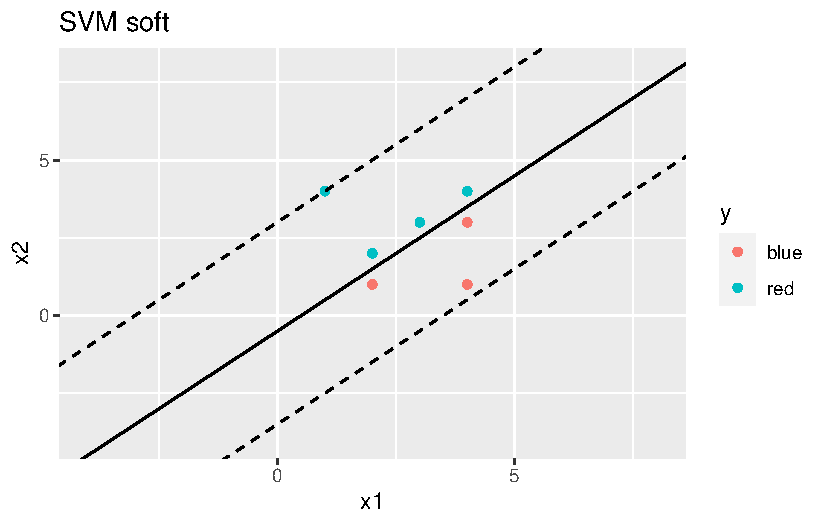
\includegraphics{excercise_doc_files/figure-pdf/unnamed-chunk-26-1.pdf}

}

\end{figure}

\begin{enumerate}
\def\labelenumi{(\alph{enumi})}
\setcounter{enumi}{5}
\item
  Mark data points with positive slack variables ϵ.
\item
  Sketch what happens to the canonical hyperplanes with increases in C
  and decreases in C, and discuss how this is related to the
  bias-variance trade-off.
\end{enumerate}

With too increased C our canonical hyperplanes includes large distance
to each observation and will include more misclassified observation.
With the right amount increase in C will create a more robust model the
could increse the performance of the model in the testing data.

\hypertarget{checkpoint-18-regularization}{%
\subsection{Checkpoint 18:
Regularization}\label{checkpoint-18-regularization}}

\begin{enumerate}
\def\labelenumi{(\alph{enumi})}
\item
  Provide a sketch of typical training error and test error on a single
  plot, as a function of the regularization parameter C. C should be on
  the x-axis, and the y-axis should represent the values for each curve.
\item
  Explain why each of the two curves has the shape displayed in (a)
  (Hint: see g in the previous checkpoint).
\end{enumerate}

\emph{With the right amount increase in C will create a more robust
model the could increase the performance of the model in the testing
data. But with too high C, too much error rate are introduced and more
misclassification occur.}

\begin{enumerate}
\def\labelenumi{(\alph{enumi})}
\setcounter{enumi}{2}
\tightlist
\item
  Explain how a suitable amount of regularization is chosen in a
  real-world application.
\end{enumerate}

\emph{Where C has decreased the error rate in testing dataset and are
not too increased in the training dataset.}

\hypertarget{checkpoint-19-support-vector-machine-aka.-kernel-svm-or-non-linear-svm}{%
\subsection{Checkpoint 19: Support vector machine (aka. kernel SVM or
non-linear
SVM)}\label{checkpoint-19-support-vector-machine-aka.-kernel-svm-or-non-linear-svm}}

\begin{enumerate}
\def\labelenumi{(\alph{enumi})}
\item
  Describe a scenario where use of a non-linear SVM may lead to better
  performance relative to a linear classifier.
\item
  What is a kernel function?
\end{enumerate}

\emph{How much we want to expand our feature space. We can when make
non-linear decision boundaries.}

\begin{enumerate}
\def\labelenumi{(\alph{enumi})}
\setcounter{enumi}{2}
\tightlist
\item
  Describe what an evaluation of the kernel function corresponds to.
\end{enumerate}

\hypertarget{checkpoint-20-support-vector-machine---csf-biomarker-data}{%
\subsection{Checkpoint 20: Support vector machine - CSF biomarker
data}\label{checkpoint-20-support-vector-machine---csf-biomarker-data}}

In this checkpoint you will analyse the CSF biomarker data using a
support vector classifier (soft-margin SVM). The goal of the analysis is
to build a support vector machine to predict group membership
(control/impaired) based on 130 CSF features. • Open the script main4a.m
/ main4a.R and review it to understand the different steps in the
script. Use the script to answer the following:

\begin{enumerate}
\def\labelenumi{(\alph{enumi})}
\tightlist
\item
  Load the data set csfBiomarkers.txt. Describe the data, what is the
  size of the data set? how many observations and features?
\end{enumerate}

\emph{131 observation and 131 features}

\begin{enumerate}
\def\labelenumi{(\alph{enumi})}
\setcounter{enumi}{1}
\tightlist
\item
  Identify the part of the script where the random partition is
  performed. How many folds are used in the k-fold cross-validation?
\end{enumerate}

\emph{10 K-folds}

\begin{enumerate}
\def\labelenumi{(\alph{enumi})}
\setcounter{enumi}{2}
\tightlist
\item
  Identify the part of the script where the range of the regularization
  parameter C is defined. Which sequence of C-values is used?
\end{enumerate}

\emph{Cvalues = 2\^{}seq(15, 0, by = -0.5)}

\begin{enumerate}
\def\labelenumi{(\alph{enumi})}
\setcounter{enumi}{3}
\tightlist
\item
  The script contains two for-loops (one nested within the other).
  Explain, in your own words, how the analysis is performed/structured
  in the script.
\end{enumerate}

\emph{The first loop includes making the traing and the testing data set
by 10 K-fold. The second loop includes the supporting vector machine
function to train the model based on the traning data set and different
sequnece of C-values. Afterwards the trained model are evaluated the
classifier performance and error rate both on the training data and the
testing data.}

\begin{enumerate}
\def\labelenumi{(\alph{enumi})}
\setcounter{enumi}{4}
\tightlist
\item
  The function fitcsvm (Matlab) svm (R) is here used to fit the SVM.
  Describe the input parameter C.
\end{enumerate}

\emph{C defines the contraining limits for flexibility of the model
epsilon distance. In the svm function, we are looping with the sequence
of different constraining values.}

\begin{enumerate}
\def\labelenumi{(\alph{enumi})}
\setcounter{enumi}{5}
\tightlist
\item
  Run the analysis. Plot the training error and the test error as a
  function of the regularization parameter C. Include the plot in your
  report and describe/discuss it. Also discuss the curves in terms of
  the bias-variance trade-off. How would you choose the ``best'' model?
  For the selected model report the training and test error.
\end{enumerate}

\begin{Shaded}
\begin{Highlighting}[]
\CommentTok{\#|include: false}
\FunctionTok{source}\NormalTok{(}\FunctionTok{here}\NormalTok{(}\StringTok{"R/day\_2\_code/main4a.R"}\NormalTok{))}
\end{Highlighting}
\end{Shaded}

\begin{verbatim}
[1] "cross-validation iteration 1 of 10"
[1] "cross-validation iteration 2 of 10"
[1] "cross-validation iteration 3 of 10"
[1] "cross-validation iteration 4 of 10"
[1] "cross-validation iteration 5 of 10"
[1] "cross-validation iteration 6 of 10"
[1] "cross-validation iteration 7 of 10"
[1] "cross-validation iteration 8 of 10"
[1] "cross-validation iteration 9 of 10"
[1] "cross-validation iteration 10 of 10"
[1] "best C: log2(C)=6.500"
training error: 0.061087788616validation error: 0.120202020202

rank                                feature beta_med        beta_mean
1                                  VEGF 0.1352211609117568  0.1360782514540126
2                                   tau 0.1313319087911661  0.1338873372707146
3                                 Ab_42 0.1186144557403955  0.1158173630445215
4                                 p_tau 0.1075343239613879  0.1045507794826668
5                Pancreatic_polypeptide 0.1007222132466663  0.0994546719441395
6                                 APOE4 0.0992789600479545  0.1000455766732265
7                                   FAS 0.0860804376143032  0.0870808319358136
8                             TGF_alpha 0.0801352411817604  0.0790962578965742
9                     Apolipoprotein_A1 0.0767218226497711  0.0752290629478989
10     Gamma_Interferon_induced_Monokin 0.0743071935340704  0.0746875720555074
11                           Fas_Ligand 0.0674970357612631  0.0661627962697078
12                                 MMP7 0.0674760161383647  0.0649619586303775
13                                  CgA 0.0665078078713796  0.0665089848653532
14                               Leptin 0.0651142398516748  0.0610011684504967
15                       Thrombopoietin 0.0624202269109118  0.0615451703150764
16                          Vitronectin 0.0611453376637200  0.0602860642684041
17                 Angiopoietin_2_ANG_2 0.0608584712171963  0.0612079633763858
18     Pulmonary_and_Activation_Regulat 0.0605090124005823  0.0596292862858354
19                             TRAIL_R3 0.0600289207332624  0.0608171577959081
20      Thymus_Expressed_Chemokine_TECK 0.0573802222051441  0.0580284462240219
21                                 IL_8 0.0560148252101107  0.0548975948875549
22                                 SGOT 0.0539850548360047  0.0512301609186281
23                                  MIF 0.0531026624245912  0.0510490792737252
24                Alpha_1_Microglobulin 0.0509380481959449  0.0511191277073620
25                          Adiponectin 0.0506373771835833  0.0554136608419015
26                                MMP_2 0.0502657671402938  0.0499650690547222
27                              Insulin 0.0482905089784778  0.0484060537193373
28                          Osteopontin 0.0473992534670606  0.0484008631479224
29       Kidney_Injury_Molecule_1_KIM_1 0.0458138798413209  0.0472538857397443
30                                IL_13 0.0457889376798449  0.0428265061062505
31           Fatty_Acid_Binding_Protein 0.0452012902917634  0.0457413577222826
32                           MIP_1alpha 0.0448646049384418  0.0471029241916073
33                     Apolipoprotein_E 0.0442374102843155  0.0447729433856427
34      Glutathione_S_Transferase_alpha 0.0431663170356018  0.0433722399086458
35                             Cortisol 0.0422914754145716  0.0399160218756554
36           Thyroxine_Binding_Globulin 0.0417497275077478  0.0404067501116882
37                               ENA_78 0.0416301589127375  0.0421026111132036
38                                 male 0.0413316859377936  0.0428544064177807
39                              TNF_RII 0.0411381537456939  0.0408388221161413
40                          Transferrin 0.0394637511079006  0.0405012432907120
41                                NrCAM 0.0392175628431130  0.0397307318496449
42                                LOX_1 0.0388350082483308  0.0377355100000994
43                                IL_11 0.0388083024727003  0.0398211019742044
44      Connective_Tissue_Growth_Factor 0.0379803508876936  0.0396420440592913
45                        Lipoprotein_a 0.0374768209203969  0.0362862072258362
46                              EN_RAGE 0.0363152749193788  0.0372348194090619
47                            Protein_S 0.0339535172819322  0.0360886509825811
48                           Cystatin_C 0.0338289701812636  0.0348105563517363
49                                  IgA 0.0333282866496066  0.0327011835115190
50           Prostatic_Acid_Phosphatase 0.0330017799334099  0.0311967438297062
51                                  PYY 0.0325627318249369  0.0334640894349882
52                               RANTES 0.0318127659400429  0.0324911655174410
53                                MCP_2 0.0315066761422801  0.0294577837711966
54                             Sortilin 0.0307554337876255  0.0306638590071392
55                               HB_EGF 0.0297722507889306  0.0292705416860247
56                           Calcitonin 0.0284855156657966  0.0263394786009990
57                            GRO_alpha 0.0280567922119672  0.0297435874377882
58                von_Willebrand_Factor 0.0272053328024014  0.0263059972959384
59                                PAI_1 0.0269403659571752  0.0276450017800953
60                    Apolipoprotein_A2 0.0259396359510833  0.0261851033106252
61                      Angiotensinogen 0.0259173874593059  0.0283081022948019
62                     Apolipoprotein_B 0.0257334878604043  0.0276467580392318
63                                MMP10 0.0255429395804255  0.0250638157340718
64                            NT_proBNP 0.0250706840124769  0.0280620787009331
65                                HCC_4 0.0248887614439854  0.0233867068092644
66                            MIP_1beta 0.0248641854590307  0.0243276531272495
67                                  AXL 0.0233020838712435  0.0243041786536506
68                                 IL_6 0.0222624615067021  0.0215794515042835
69                               PAPP_A 0.0221680257937659  0.0220787746973861
70      B_Lymphocyte_Chemoattractant_BL 0.0215241849730477  0.0207970216470741
71         Hepatocyte_Growth_Factor_HGF 0.0212804767986699  0.0224543973397779
72                       Thrombomodulin 0.0210077992236182  0.0193389282730406
73                                  age 0.0204666698081446  0.0206019935346952
74                         Betacellulin 0.0199226188829317  0.0200984074964781
75                Alpha_2_Macroglobulin 0.0199131555292193  0.0194367165993934
76                                S100b 0.0195334831754275  0.0177126682238445
77                Trefoil_Factor_3_TFF3 0.0189961893594835  0.0167111380381539
78                             IGF_BP_2 0.0183841219237350  0.0183482534632324
79                   C_Reactive_Protein 0.0180991764065553  0.0180492525523555
80                     Apolipoprotein_H 0.0168152389737655  0.0197131166945776
81                     Stem_Cell_Factor 0.0167154099286166  0.0165753055202758
82                                 PLGF 0.0162710186163791  0.0137022542416678
83       ACE_CD143_Angiotensin_Converti 0.0147582118548362  0.0173993299292211
84             Alpha_1_Antichymotrypsin 0.0147218166603414  0.0137674258489347
85                               TIMP_1 0.0145487404481964  0.0114758328997816
86                                BMP_6 0.0144099543294745  0.0134767083918962
87                                MCP_1 0.0141913884274159  0.0177503651614498
88           IP_10_Inducible_Protein_10 0.0134894375974933  0.0119018018366286
89                                EGF_R 0.0134035420601307  0.0136771594627240
90                            Calbindin 0.0128852339500894  0.0107102920715260
91                           Fibrinogen 0.0128524288287225  0.0125245392594695
92                         Complement_3 0.0128338058871559  0.0134338320798326
93                   Creatine_Kinase_MB 0.0123885148663913  0.0134836989702317
94                                 IL_7 0.0123689881924617  0.0157712086321971
95                             Resistin 0.0122770209736833  0.0118103808480105
96                                 IL_3 0.0119178617784431  0.0120800349009855
97                                MMP_3 0.0115639908973920  0.0119040986687776
98          Thyroid_Stimulating_Hormone 0.0111564908406895  0.0077868511672867
99                  Apolipoprotein_CIII 0.0107978621714940  0.0095610651286564
100                            Ferritin 0.0097191047668033  0.0081279068343400
101                           Eotaxin_3 0.0095095985184020  0.0094427492056264
102                            Fetuin_A 0.0090790763038669  0.0104873783714443
103                                CD5L 0.0090386962608050  0.0109093482688162
104                              IL_17E 0.0089448043227913  0.0097482338382546
105                                IL_4 0.0089110702626683  0.0093936262083889
106                 Complement_Factor_H 0.0082993348463485  0.0095751982775259
107                   Apolipoprotein_CI 0.0072901725492028  0.0065009038762004
108           Tamm_Horsfall_Protein_THP 0.0072382759015357  0.0057881161336375
109                                IL_5 0.0065916223213170  0.0099586373648100
110                              VCAM_1 0.0064273692816414  0.0077864682117073
111                 Apolipoprotein_A_IV 0.0060475166953474  0.0082047026158635
112                           IL_1alpha 0.0056351141059563  0.0052386284313642
113                 Alpha_1_Antitrypsin 0.0055460539803515  0.0025998628012837
114                                SHBG 0.0047108554861490  0.0061675883205274
115                      TTR_prealbumin 0.0043269190266427  0.0061807173731264
116                              ICAM_1 0.0041092958479461  0.0000379554935495
117     FSH_Follicle_Stimulation_Hormon 0.0039162148301439  0.0041367033406627
118                           Prolactin 0.0032683105632894  0.0016517234328270
119                    Apolipoprotein_D 0.0031715541324877  0.0038749569143538
120                                 SOD 0.0030932180290735  0.0018234972682437
121                           Myoglobin 0.0024864471088579  0.0037167765534672
122                     Serum_Amyloid_P 0.0023833931054960  0.0033321427246064
123                       Tissue_Factor 0.0022704683387498  0.0024179800394612
124     ACTH_Adrenocorticotropic_Hormon 0.0021514129012410  0.0012423757440879
125                                CD40 0.0019275145860677  0.0010948238505909
126                     Clusterin_Apo_J 0.0014609881526506  0.0002723624709005
127                       IL_6_Receptor 0.0013811875191219  0.0024706808294852
128                               IL_16 0.0010428678160593  0.0000758430763493
129                Beta_2_Microglobulin 0.0003624839198170  0.0018110132072159
130                               I_309 0.0001458200548108  0.0007150844221072
\end{verbatim}

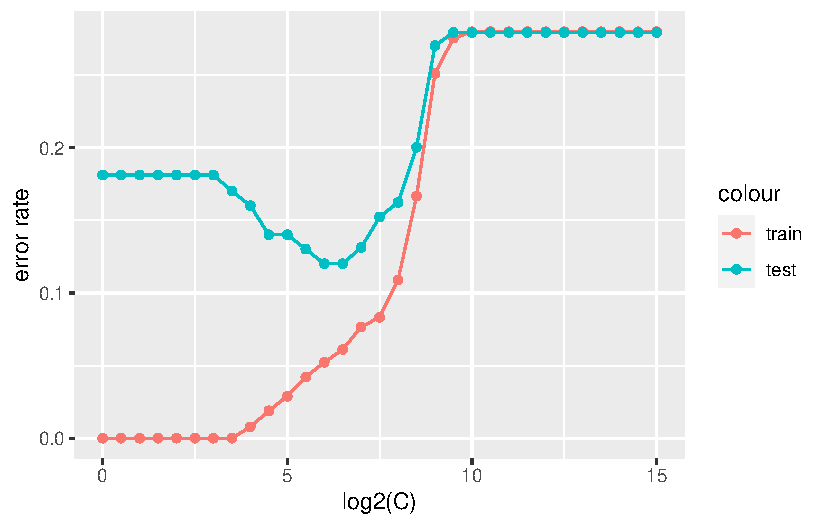
\includegraphics{excercise_doc_files/figure-pdf/unnamed-chunk-28-1.pdf}

\begin{verbatim}
with higher C values error rate in testing data set deacrease until at some point near log(C) = 6. Hence, I would choose a odel fittet with a log(C) values at 6.
\end{verbatim}

\begin{enumerate}
\def\labelenumi{(\alph{enumi})}
\setcounter{enumi}{6}
\item
  Look at the β coefficient array. What is the dimensionality of β?
\item
  Include the plot with coefficient traces as a function of C in your
  report and describe/discuss it. What happens with coefficients with
  decreased model complexity/ regularization strength? Are any
  coefficients exactly zero? Look at the coefficients for your chosen
  model. Identify the most important coefficients to the model.

  The coefficens values for the model are shrinkaging by higher C value,
  and the model become more simple. At log(C) = 6 the, the coefficients
  are slightly deminished.
\item
  Include the plot with the number of support vectors as a function of C
  in your report and describe/discuss it.
\end{enumerate}

\begin{Shaded}
\begin{Highlighting}[]
\FunctionTok{plot}\NormalTok{(plot\_sv)}
\end{Highlighting}
\end{Shaded}

\begin{figure}[H]

{\centering 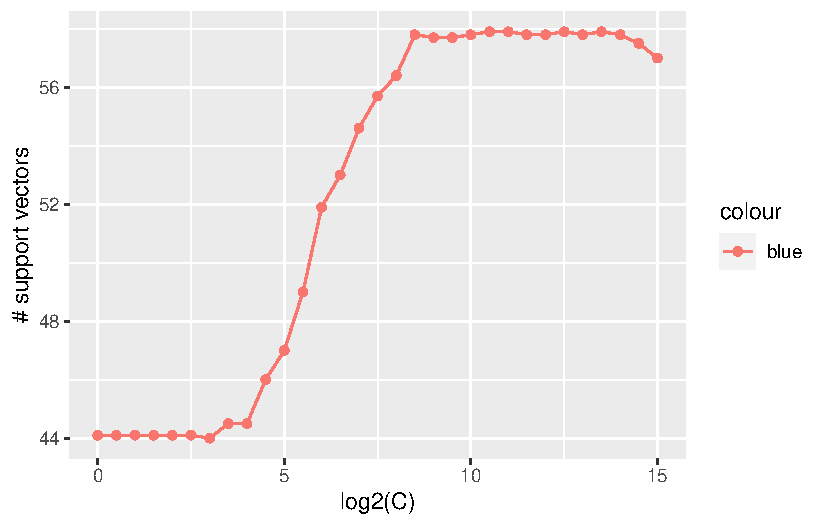
\includegraphics{excercise_doc_files/figure-pdf/unnamed-chunk-29-1.pdf}

}

\end{figure}

\begin{verbatim}
Increase of C includes more supporting vectors, which make sence bacuase the margin increases.
\end{verbatim}

\begin{enumerate}
\def\labelenumi{(\alph{enumi})}
\setcounter{enumi}{9}
\tightlist
\item
  Plot the confusion matrix for your chosen model. Include it in your
  report and describe/discuss it. Based on the numbers in the confusion
  matrix, compute and report the following performance metrics for the
  test set: classification accuracy, error rate, true positive rate,
  true negative rate, false positive rate, false negative rate,
  sensitivity, and specificity.
\end{enumerate}

\begin{Shaded}
\begin{Highlighting}[]
\NormalTok{m\_rates\_train}
\end{Highlighting}
\end{Shaded}

\begin{verbatim}
         control impaired
imparied      52      200
control      645        3
\end{verbatim}

\begin{Shaded}
\begin{Highlighting}[]
\FunctionTok{evaluation\_matrix}\NormalTok{(m\_rates\_train[}\DecValTok{1}\NormalTok{,}\DecValTok{2}\NormalTok{],m\_rates\_train[}\DecValTok{1}\NormalTok{,}\DecValTok{2}\NormalTok{],m\_rates\_train[}\DecValTok{1}\NormalTok{,}\DecValTok{1}\NormalTok{],m\_rates\_train[}\DecValTok{2}\NormalTok{,}\DecValTok{2}\NormalTok{])}
\end{Highlighting}
\end{Shaded}

\begin{verbatim}
       true_pr  false_pr   true_nr   false_nr      sens      spec
[1,] 0.7936508 0.2063492 0.9852217 0.01477833 0.9852217 0.7936508
\end{verbatim}

\begin{Shaded}
\begin{Highlighting}[]
\NormalTok{m\_rates\_test}
\end{Highlighting}
\end{Shaded}

\begin{verbatim}
         control impaired
imparied       9       19
control       69        3
\end{verbatim}

\begin{Shaded}
\begin{Highlighting}[]
\FunctionTok{evaluation\_matrix}\NormalTok{(m\_rates\_test[}\DecValTok{1}\NormalTok{,}\DecValTok{2}\NormalTok{],m\_rates\_test[}\DecValTok{1}\NormalTok{,}\DecValTok{2}\NormalTok{],m\_rates\_test[}\DecValTok{1}\NormalTok{,}\DecValTok{1}\NormalTok{],m\_rates\_test[}\DecValTok{2}\NormalTok{,}\DecValTok{2}\NormalTok{])}
\end{Highlighting}
\end{Shaded}

\begin{verbatim}
       true_pr  false_pr   true_nr  false_nr      sens      spec
[1,] 0.6785714 0.3214286 0.8636364 0.1363636 0.8636364 0.6785714
\end{verbatim}

\hypertarget{neural-networks}{%
\section{8 Neural networks}\label{neural-networks}}

\hypertarget{checkpoint-21-bneural-networks-vs.-linear--and-logistic-regression}{%
\subsection{Checkpoint 21: bNeural networks vs.~linear- and logistic
regression}\label{checkpoint-21-bneural-networks-vs.-linear--and-logistic-regression}}

\begin{enumerate}
\def\labelenumi{(\alph{enumi})}
\item
  Discuss limitations of linear regression and logistic regression and
  possible advantages of neural networks.

  Can't handle other complex data e.g.~imaging, text, sound,
  time-series. Thus, the models can't train test and clissify based on
  other than tabular data often measured cross-sectionally.
\end{enumerate}

\hypertarget{checkpoint-22-design-a-neural-network}{%
\section{Checkpoint 22: Design a neural
network}\label{checkpoint-22-design-a-neural-network}}

Think of a classification task where the feature dimensionality is two
and there are two possible classes (binary classification). The aim of
this checkpoint is to draw a graphical representation of a NN with one
hidden layer containing three hidden nodes.

\begin{enumerate}
\def\labelenumi{(\alph{enumi})}
\item
  Begin with drawing input nodes, how many input nodes?

  2 inpute beacuase we have two features.
\item
  Add hidden nodes to your sketch and draw connections between input
  nodes and the hidden nodes.

  check
\item
  Add a bias node your sketch and draw connections between this bias
  node and the hidden nodes.

  check
\item
  Add two output nodes to the sketch. Draw connections between hidden
  nodes and the output nodes. check
\item
  Add another bias node your sketch and draw connections between this
  bias node and the output node.

  check
\item
  How are the inputs to each of the hidden nodes computed? Write down
  the formula for the input to a hidden node.
\end{enumerate}

\emph{compute activation} Ak = g(wk0 + sum\_p\_j=1(wkj*Xj))

\begin{enumerate}
\def\labelenumi{(\alph{enumi})}
\setcounter{enumi}{6}
\tightlist
\item
  Explain what a hidden node activation function is. Write down the
  formula fora ReLU activation function and make a sketch of hidden node
  output/activation Ak as a function of its input zk.
\end{enumerate}

Hidden node activation is how the hidden unit are responding to a
particular set of input, hence creating the weight path from the set of
hidden notes to predict the outcome.

f(x) = B0 + sum\_k\_k=1(Bk*Ak)

\begin{enumerate}
\def\labelenumi{(\alph{enumi})}
\setcounter{enumi}{7}
\item
  How are the inputs to the output nodes computed. Write down the
  formula for the inputs to the output nodes.

  Add description f(x) = sum\_K\_K=1(Bk\emph{g(wk0 +
  sum\_p\_j=1(wkj}Xj)))
\item
  We will use the softmax activation function for the model's output.
  Describe what the network's two outputs represent. What is the
  numerical range of the outputs, and how can the network's outputs be
  interpreted?
\item
  Can this network produce non-linear decision boundaries? (Hint:
  Consider whether linear or non-linear activation functions are used
  and the network architecture?).
\end{enumerate}

\hypertarget{checkpoint-23-neural-networks---regularization}{%
\subsection{Checkpoint 23: Neural networks -
regularization}\label{checkpoint-23-neural-networks---regularization}}

\begin{enumerate}
\def\labelenumi{(\alph{enumi})}
\item
  Explain when and why it may be necessary to use model regularization
  in neural networks.

  To mimimize residual error in the trained thetas (weights), and hence
  improve performace of the traing and testing data.
\item
  Write down a cost function comprising the error function and a penalty
  term that penalizes the squared weight values (Hint: See equations
  10.14 and 10.31 in ISL). Explain the meaning of two terms in this
  expression.

\begin{verbatim}
We want
With the regularitation we keep the architecture of the model, and impoving wieght by minimizing the error.
\end{verbatim}
\item
  Compare the expression in (b) with the cost function in ridge
  regularized logistic regression.
\item
  Explain how a suitable value for the regularization parameter λ can be
  chosen.

  Similiar when the error rate are lowest for both training and testing
  data set
\end{enumerate}

\hypertarget{checkpoint-24-neural-network---csf-biomarker-data}{%
\subsection{Checkpoint 24: Neural network - CSF biomarker
data}\label{checkpoint-24-neural-network---csf-biomarker-data}}

In this checkpoint you will analyse the CSF biomarker data using a
feed-forward neural network. The goal of the analysis is to build a
neural network to predict group membership (control/impaired) based on
130 CSF features.

• Open the script main5a.m / main5a.R and review it to understand the
different steps in the script. Use the script to answer the following:

\begin{enumerate}
\def\labelenumi{(\alph{enumi})}
\item
  Load the data set csfBiomarkers.txt. Describe the data, what is the
  size of the data set? how many observations and features?

  100 obs and 131 variables
\item
  Describe the neural network architecture. How many hidden nodes and
  hidden layers?

  The NN are based on 2 hidden layers and 8 hidden nodes, and 131
  inputs.
\item
  Make a sketch showing the structure of this neural network. What is
  the number of parameters in the neural network?

  insert figure
\end{enumerate}

\begin{Shaded}
\begin{Highlighting}[]
\NormalTok{parameters }\OtherTok{\textless{}{-}} \DecValTok{131}\SpecialCharTok{*}\DecValTok{8}\SpecialCharTok{+}\DecValTok{8}\SpecialCharTok{*}\DecValTok{8}\SpecialCharTok{+}\DecValTok{8}\SpecialCharTok{*}\DecValTok{8}\SpecialCharTok{+}\DecValTok{1}\SpecialCharTok{*}\DecValTok{8}\SpecialCharTok{+}\DecValTok{1}\SpecialCharTok{*}\DecValTok{8}\SpecialCharTok{+}\DecValTok{1}\SpecialCharTok{*}\DecValTok{8}
\NormalTok{parameters}
\end{Highlighting}
\end{Shaded}

\begin{verbatim}
[1] 1200
\end{verbatim}

\begin{enumerate}
\def\labelenumi{(\alph{enumi})}
\setcounter{enumi}{3}
\item
  Identify the part of the script where the random partition is
  performed. How many folds are used in the k-fold cross-validation?

  10 folds
\item
  Identify the part of the script where the range of the regularization
  parameter λ is defined. Which sequence of λ-values is used?

  2\^{}seq(-12, 5, by = 1)
\item
  The script contains two for-loops (one nested within the other).
  Explain, in your own words, how the analysis is performed/structured
  in the script.

  The first part is splitting the data into train and test by k folds.
  The second part, is to rund the neural network
\item
  Run the analysis. Plot the training error and the test error as a
  function of the regularization parameter λ. Include the plot in your
  report and describe/discuss it. Also discuss the curves in terms of
  the bias-variance trade-off. How would you choose the ``best'' model?
  For the selected model report the training and test error.

  I will chose model with log(lambda) = -5, because it has the best
  performance in error rate in traning and test set combined. I assume
  that the bias has decreased, and variance has increased, which give a
  small increase in training dataset. However the sweetspot between
  these can be found at -5.
\end{enumerate}

\begin{Shaded}
\begin{Highlighting}[]
\CommentTok{\#source(here("R/day\_3\_code/main5a.R"))}
\CommentTok{\#plot(error\_plot)}
\end{Highlighting}
\end{Shaded}

\begin{enumerate}
\def\labelenumi{(\alph{enumi})}
\setcounter{enumi}{7}
\item
  Can we interpret the weights/coefficients of a neural network in the
  same way as we did for logistic regression? Can we identify important
  features by looking at the weights directly?

  No, we can't, as we cant interpret the hidden weights in the hidden
  layers. Maybe thorugh more advanced exploration it will be possible.
\item
  Plot the confusion matrix for your chosen model. Include it in your
  report and describe/discuss it. Based on the numbers in the confusion
  matrix, compute and report the following performance metrics for the
  test set: classification accuracy, error rate, true positive rate,
  true negative rate, false positive rate, false negative rate,
  sensitivity, and specificity.
\end{enumerate}

\hypertarget{checkpoint-25-neural-networks-challenges}{%
\subsection{Checkpoint 25: Neural networks,
challenges}\label{checkpoint-25-neural-networks-challenges}}

\begin{enumerate}
\def\labelenumi{(\alph{enumi})}
\tightlist
\item
  Discuss challenges with neural networks.
\end{enumerate}

\hypertarget{pca}{%
\section{PCA}\label{pca}}

\hypertarget{checkpoint-26-pca---using-principal-components}{%
\subsection{Checkpoint 26: PCA - using principal
components}\label{checkpoint-26-pca---using-principal-components}}

Suppose that we have the following five data points in R3 (3-dimensional
data) x1 x2 x3 x4 x5 xi1 -2 -2 0 2 2 xi2 -2 2 0 -2 2 xi3 -4 0 0 0 4 The
variables in this data set has zero mean. Principal component analysis
of the data set has provided the following three vectors ϕ1 = (0.41,
0.41, 0.82)T , ϕ2 = (−0.71, 0.71, 0.00)T and ϕ3 = (0.58, 0.58,−0.58)T.

\begin{enumerate}
\def\labelenumi{(\alph{enumi})}
\tightlist
\item
  Calculate and report the principal component scores zi1, zi2, and zi3
  for each of the five data points.
\end{enumerate}

\begin{Shaded}
\begin{Highlighting}[]
\NormalTok{zi }\OtherTok{\textless{}{-}} \ControlFlowTok{function}\NormalTok{(x1,x2,x3,o11,o12,o13)}
\NormalTok{\{}
\NormalTok{    z }\OtherTok{=}\NormalTok{ x1}\SpecialCharTok{*}\NormalTok{o11 }\SpecialCharTok{+}\NormalTok{ x2}\SpecialCharTok{*}\NormalTok{o12 }\SpecialCharTok{+}\NormalTok{ x3}\SpecialCharTok{*}\NormalTok{o13}

        \FunctionTok{return}\NormalTok{(z)}
\NormalTok{\}}


\CommentTok{\# x1}
\NormalTok{x1 }\OtherTok{\textless{}{-}}  \FunctionTok{c}\NormalTok{(}\SpecialCharTok{{-}}\DecValTok{2}\NormalTok{,}\SpecialCharTok{{-}}\DecValTok{2}\NormalTok{,}\SpecialCharTok{{-}}\DecValTok{4}\NormalTok{)}

\NormalTok{z11}\OtherTok{\textless{}{-}} \FunctionTok{zi}\NormalTok{(}\SpecialCharTok{{-}}\DecValTok{2}\NormalTok{,}\SpecialCharTok{{-}}\DecValTok{2}\NormalTok{,}\SpecialCharTok{{-}}\DecValTok{4}\NormalTok{, }\FloatTok{0.41}\NormalTok{, }\FloatTok{0.41}\NormalTok{, }\FloatTok{0.82}\NormalTok{) }\CommentTok{\# z1}
\NormalTok{z21 }\OtherTok{\textless{}{-}} \FunctionTok{zi}\NormalTok{(}\SpecialCharTok{{-}}\DecValTok{2}\NormalTok{,}\SpecialCharTok{{-}}\DecValTok{2}\NormalTok{,}\SpecialCharTok{{-}}\DecValTok{4}\NormalTok{, }\SpecialCharTok{{-}}\FloatTok{0.71}\NormalTok{, }\FloatTok{0.71}\NormalTok{, }\FloatTok{0.00}\NormalTok{)}\CommentTok{\# z2}
\NormalTok{z31 }\OtherTok{\textless{}{-}} \FunctionTok{zi}\NormalTok{(}\SpecialCharTok{{-}}\DecValTok{2}\NormalTok{,}\SpecialCharTok{{-}}\DecValTok{2}\NormalTok{,}\SpecialCharTok{{-}}\DecValTok{4}\NormalTok{, }\FloatTok{0.58}\NormalTok{, }\FloatTok{0.58}\NormalTok{, }\SpecialCharTok{{-}}\FloatTok{0.58}\NormalTok{)}\CommentTok{\# z3}

\CommentTok{\# x2}
\NormalTok{z12}\OtherTok{\textless{}{-}} \FunctionTok{zi}\NormalTok{(}\SpecialCharTok{{-}}\DecValTok{2}\NormalTok{,}\DecValTok{2}\NormalTok{,}\DecValTok{0}\NormalTok{, }\FloatTok{0.41}\NormalTok{, }\FloatTok{0.41}\NormalTok{, }\FloatTok{0.82}\NormalTok{) }\CommentTok{\# z1}
\NormalTok{z22 }\OtherTok{\textless{}{-}}\FunctionTok{zi}\NormalTok{(}\SpecialCharTok{{-}}\DecValTok{2}\NormalTok{,}\DecValTok{2}\NormalTok{,}\DecValTok{0}\NormalTok{, }\SpecialCharTok{{-}}\FloatTok{0.71}\NormalTok{, }\FloatTok{0.71}\NormalTok{, }\FloatTok{0.00}\NormalTok{)}\CommentTok{\# z2}
\NormalTok{z32 }\OtherTok{\textless{}{-}}\FunctionTok{zi}\NormalTok{(}\SpecialCharTok{{-}}\DecValTok{2}\NormalTok{,}\DecValTok{2}\NormalTok{,}\DecValTok{0}\NormalTok{, }\FloatTok{0.58}\NormalTok{, }\FloatTok{0.58}\NormalTok{, }\SpecialCharTok{{-}}\FloatTok{0.58}\NormalTok{)}\CommentTok{\# z3}

\CommentTok{\# x3}
\NormalTok{z13}\OtherTok{\textless{}{-}} \FunctionTok{zi}\NormalTok{(}\DecValTok{0}\NormalTok{,}\DecValTok{0}\NormalTok{,}\DecValTok{0}\NormalTok{, }\FloatTok{0.41}\NormalTok{, }\FloatTok{0.41}\NormalTok{, }\FloatTok{0.82}\NormalTok{) }\CommentTok{\# z1}
\NormalTok{z23 }\OtherTok{\textless{}{-}}\FunctionTok{zi}\NormalTok{(}\DecValTok{0}\NormalTok{,}\DecValTok{0}\NormalTok{,}\DecValTok{0}\NormalTok{, }\SpecialCharTok{{-}}\FloatTok{0.71}\NormalTok{, }\FloatTok{0.71}\NormalTok{, }\FloatTok{0.00}\NormalTok{)}\CommentTok{\# z2}
\NormalTok{z33 }\OtherTok{\textless{}{-}}\FunctionTok{zi}\NormalTok{(}\DecValTok{0}\NormalTok{,}\DecValTok{0}\NormalTok{,}\DecValTok{0}\NormalTok{, }\FloatTok{0.58}\NormalTok{, }\FloatTok{0.58}\NormalTok{, }\SpecialCharTok{{-}}\FloatTok{0.58}\NormalTok{)}\CommentTok{\# z3}


\CommentTok{\# x4}
\NormalTok{z14 }\OtherTok{\textless{}{-}} \FunctionTok{zi}\NormalTok{(}\DecValTok{2}\NormalTok{,}\SpecialCharTok{{-}}\DecValTok{2}\NormalTok{,}\DecValTok{0}\NormalTok{, }\FloatTok{0.41}\NormalTok{, }\FloatTok{0.41}\NormalTok{, }\FloatTok{0.82}\NormalTok{)}\CommentTok{\# z1}
\NormalTok{z24 }\OtherTok{\textless{}{-}}\FunctionTok{zi}\NormalTok{(}\DecValTok{2}\NormalTok{,}\SpecialCharTok{{-}}\DecValTok{2}\NormalTok{,}\DecValTok{0}\NormalTok{, }\SpecialCharTok{{-}}\FloatTok{0.71}\NormalTok{, }\FloatTok{0.71}\NormalTok{, }\FloatTok{0.00}\NormalTok{)}\CommentTok{\# z2}
\NormalTok{z34 }\OtherTok{\textless{}{-}}\FunctionTok{zi}\NormalTok{(}\DecValTok{2}\NormalTok{,}\SpecialCharTok{{-}}\DecValTok{2}\NormalTok{,}\DecValTok{0}\NormalTok{, }\FloatTok{0.58}\NormalTok{, }\FloatTok{0.58}\NormalTok{, }\SpecialCharTok{{-}}\FloatTok{0.58}\NormalTok{)}\CommentTok{\# z3}

\CommentTok{\# x5}

\NormalTok{z15 }\OtherTok{\textless{}{-}}\FunctionTok{zi}\NormalTok{(}\DecValTok{2}\NormalTok{,}\DecValTok{2}\NormalTok{,}\DecValTok{4}\NormalTok{, }\FloatTok{0.41}\NormalTok{, }\FloatTok{0.41}\NormalTok{, }\FloatTok{0.82}\NormalTok{)}\CommentTok{\# z1}
\NormalTok{z25 }\OtherTok{\textless{}{-}}\FunctionTok{zi}\NormalTok{(}\DecValTok{2}\NormalTok{,}\DecValTok{2}\NormalTok{,}\DecValTok{4}\NormalTok{, }\SpecialCharTok{{-}}\FloatTok{0.71}\NormalTok{, }\FloatTok{0.71}\NormalTok{, }\FloatTok{0.00}\NormalTok{)}\CommentTok{\# z2}
\NormalTok{z35 }\OtherTok{\textless{}{-}}\FunctionTok{zi}\NormalTok{(}\DecValTok{2}\NormalTok{,}\DecValTok{2}\NormalTok{,}\DecValTok{4}\NormalTok{, }\FloatTok{0.58}\NormalTok{, }\FloatTok{0.58}\NormalTok{, }\SpecialCharTok{{-}}\FloatTok{0.58}\NormalTok{)}\CommentTok{\# z3}
\end{Highlighting}
\end{Shaded}

\begin{enumerate}
\def\labelenumi{(\alph{enumi})}
\setcounter{enumi}{1}
\tightlist
\item
  Calculate and report how big a proportion of the total variance is
  captured by each of the individual individual principal components (PV
  E1, PV E2, and PV E3). Create a scree plot from these and describe and
  comment on the plot.
\end{enumerate}

PV E1

\begin{Shaded}
\begin{Highlighting}[]
\NormalTok{PV\_E1 }\OtherTok{\textless{}{-}}\NormalTok{ (z11}\SpecialCharTok{\^{}}\DecValTok{2}\SpecialCharTok{+}\NormalTok{z12}\SpecialCharTok{\^{}}\DecValTok{2}\SpecialCharTok{+}\NormalTok{z13}\SpecialCharTok{\^{}}\DecValTok{2}\SpecialCharTok{+}\NormalTok{z14}\SpecialCharTok{\^{}}\DecValTok{2}\SpecialCharTok{+}\NormalTok{z15}\SpecialCharTok{\^{}}\DecValTok{2}\NormalTok{)}\SpecialCharTok{/}\NormalTok{(}\DecValTok{5{-}1}\NormalTok{)}
\end{Highlighting}
\end{Shaded}

\begin{Shaded}
\begin{Highlighting}[]
\NormalTok{PV\_E2 }\OtherTok{\textless{}{-}}\NormalTok{ (z21}\SpecialCharTok{\^{}}\DecValTok{2}\SpecialCharTok{+}\NormalTok{z22}\SpecialCharTok{\^{}}\DecValTok{2}\SpecialCharTok{+}\NormalTok{z23}\SpecialCharTok{\^{}}\DecValTok{2}\SpecialCharTok{+}\NormalTok{z24}\SpecialCharTok{\^{}}\DecValTok{2}\SpecialCharTok{+}\NormalTok{z25}\SpecialCharTok{\^{}}\DecValTok{2}\NormalTok{)}\SpecialCharTok{/}\NormalTok{(}\DecValTok{5{-}1}\NormalTok{)}
\end{Highlighting}
\end{Shaded}

\begin{Shaded}
\begin{Highlighting}[]
\NormalTok{PV\_E3 }\OtherTok{\textless{}{-}}\NormalTok{ (z31}\SpecialCharTok{\^{}}\DecValTok{2}\SpecialCharTok{+}\NormalTok{z32}\SpecialCharTok{\^{}}\DecValTok{2}\SpecialCharTok{+}\NormalTok{z33}\SpecialCharTok{\^{}}\DecValTok{2}\SpecialCharTok{+}\NormalTok{z34}\SpecialCharTok{\^{}}\DecValTok{2}\SpecialCharTok{+}\NormalTok{z35}\SpecialCharTok{\^{}}\DecValTok{2}\NormalTok{)}\SpecialCharTok{/}\NormalTok{(}\DecValTok{5{-}1}\NormalTok{)}
\end{Highlighting}
\end{Shaded}

\begin{Shaded}
\begin{Highlighting}[]
\NormalTok{tot\_var }\OtherTok{\textless{}{-}} \FunctionTok{matrix}\NormalTok{(}\FunctionTok{c}\NormalTok{(}\DecValTok{1}\NormalTok{,}\DecValTok{2}\NormalTok{,}\DecValTok{3}\NormalTok{,PV\_E1,PV\_E2,PV\_E3), }\AttributeTok{nrow=}\DecValTok{3}\NormalTok{)}
\end{Highlighting}
\end{Shaded}

\begin{Shaded}
\begin{Highlighting}[]
\FunctionTok{matplot}\NormalTok{(tot\_var[,}\DecValTok{2}\NormalTok{], }\AttributeTok{type=}\StringTok{"l"}\NormalTok{, }\AttributeTok{xlab =} \StringTok{"zi"}
\NormalTok{        )}
\end{Highlighting}
\end{Shaded}

\begin{figure}[H]

{\centering 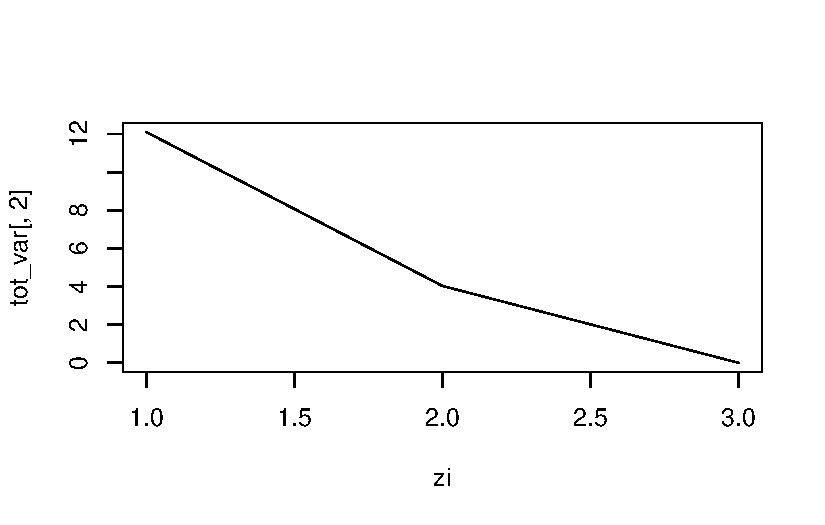
\includegraphics{excercise_doc_files/figure-pdf/unnamed-chunk-40-1.pdf}

}

\end{figure}

\begin{Shaded}
\begin{Highlighting}[]
\NormalTok{((z11}\SpecialCharTok{\^{}}\DecValTok{2}\SpecialCharTok{+}\NormalTok{z21}\SpecialCharTok{\^{}}\DecValTok{2}\SpecialCharTok{+}\NormalTok{z31}\SpecialCharTok{\^{}}\DecValTok{2}\NormalTok{)}\SpecialCharTok{/}\NormalTok{((}\SpecialCharTok{{-}}\DecValTok{2}\SpecialCharTok{\^{}}\DecValTok{2}\NormalTok{)}\SpecialCharTok{+}\NormalTok{(}\SpecialCharTok{{-}}\DecValTok{2}\SpecialCharTok{\^{}}\DecValTok{2}\NormalTok{)}\SpecialCharTok{+}\NormalTok{(}\SpecialCharTok{{-}}\DecValTok{4}\SpecialCharTok{\^{}}\DecValTok{2}\NormalTok{))) }\CommentTok{\# x1}
\end{Highlighting}
\end{Shaded}

\begin{verbatim}
[1] -1.0086
\end{verbatim}

\begin{Shaded}
\begin{Highlighting}[]
\NormalTok{((z12}\SpecialCharTok{\^{}}\DecValTok{2}\SpecialCharTok{+}\NormalTok{z22}\SpecialCharTok{\^{}}\DecValTok{2}\SpecialCharTok{+}\NormalTok{z32}\SpecialCharTok{\^{}}\DecValTok{2}\NormalTok{)}\SpecialCharTok{/}\NormalTok{((}\SpecialCharTok{{-}}\DecValTok{2}\SpecialCharTok{\^{}}\DecValTok{2}\NormalTok{)}\SpecialCharTok{+}\NormalTok{(}\DecValTok{2}\SpecialCharTok{\^{}}\DecValTok{2}\NormalTok{)}\SpecialCharTok{+}\NormalTok{(}\DecValTok{0}\SpecialCharTok{\^{}}\DecValTok{2}\NormalTok{))) }\CommentTok{\# x2}
\end{Highlighting}
\end{Shaded}

\begin{verbatim}
[1] Inf
\end{verbatim}

\begin{Shaded}
\begin{Highlighting}[]
\NormalTok{((z13}\SpecialCharTok{\^{}}\DecValTok{2}\SpecialCharTok{+}\NormalTok{z23}\SpecialCharTok{\^{}}\DecValTok{2}\SpecialCharTok{+}\NormalTok{z33}\SpecialCharTok{\^{}}\DecValTok{2}\NormalTok{)}\SpecialCharTok{/}\NormalTok{((}\DecValTok{0}\SpecialCharTok{\^{}}\DecValTok{2}\NormalTok{)}\SpecialCharTok{+}\NormalTok{(}\DecValTok{0}\SpecialCharTok{\^{}}\DecValTok{2}\NormalTok{)}\SpecialCharTok{+}\NormalTok{(}\DecValTok{0}\SpecialCharTok{\^{}}\DecValTok{2}\NormalTok{))) }\CommentTok{\# x3}
\end{Highlighting}
\end{Shaded}

\begin{verbatim}
[1] NaN
\end{verbatim}

\begin{Shaded}
\begin{Highlighting}[]
\NormalTok{((z14}\SpecialCharTok{\^{}}\DecValTok{2}\SpecialCharTok{+}\NormalTok{z24}\SpecialCharTok{\^{}}\DecValTok{2}\SpecialCharTok{+}\NormalTok{z34}\SpecialCharTok{\^{}}\DecValTok{2}\NormalTok{)}\SpecialCharTok{/}\NormalTok{((}\DecValTok{2}\SpecialCharTok{\^{}}\DecValTok{2}\NormalTok{)}\SpecialCharTok{+}\NormalTok{(}\SpecialCharTok{{-}}\DecValTok{2}\SpecialCharTok{\^{}}\DecValTok{2}\NormalTok{)}\SpecialCharTok{+}\NormalTok{(}\DecValTok{0}\SpecialCharTok{\^{}}\DecValTok{2}\NormalTok{))) }\CommentTok{\# x4}
\end{Highlighting}
\end{Shaded}

\begin{verbatim}
[1] Inf
\end{verbatim}

\begin{Shaded}
\begin{Highlighting}[]
\NormalTok{((z15}\SpecialCharTok{\^{}}\DecValTok{2}\SpecialCharTok{+}\NormalTok{z25}\SpecialCharTok{\^{}}\DecValTok{2}\SpecialCharTok{+}\NormalTok{z35}\SpecialCharTok{\^{}}\DecValTok{2}\NormalTok{)}\SpecialCharTok{/}\NormalTok{((}\DecValTok{2}\SpecialCharTok{\^{}}\DecValTok{2}\NormalTok{)}\SpecialCharTok{+}\NormalTok{(}\DecValTok{2}\SpecialCharTok{\^{}}\DecValTok{2}\NormalTok{)}\SpecialCharTok{+}\NormalTok{(}\DecValTok{4}\SpecialCharTok{\^{}}\DecValTok{2}\NormalTok{))) }\CommentTok{\# x5}
\end{Highlighting}
\end{Shaded}

\begin{verbatim}
[1] 1.0086
\end{verbatim}

\begin{enumerate}
\def\labelenumi{(\alph{enumi})}
\setcounter{enumi}{2}
\tightlist
\item
  Make a plot of the five data points embedded into the 2-dimensional
  subspace that accounts for most of the variance in the data.
\end{enumerate}

\begin{enumerate}
\def\labelenumi{(\alph{enumi})}
\setcounter{enumi}{3}
\tightlist
\item
  From the embeddings in (c) compute the reconstructions of the embedded
  points (eqn. (9)). Compare these reconstructions with the original
  data points and discuss the quality/accuracy of the reconstruction.
\end{enumerate}

\hypertarget{checkpoint-27-limitations-of-pca}{%
\subsection{Checkpoint 27: Limitations of
PCA}\label{checkpoint-27-limitations-of-pca}}

\begin{enumerate}
\def\labelenumi{(\alph{enumi})}
\item
  In the figure above, we have plotted three different 2-dimensional
  data sets. Make a sketch/drawing of how you expect the scree plot to
  look for each of the three data sets. Include the drawing in your
  report and explain your answer.
\item
  For which of the data sets will the proportion of explained variance
  be largest for the first principal component? Explain your answer.
\item
  For which of the data sets would dimensionality reduction by PCA make
  most sense? Explain your answer.
\end{enumerate}

\hypertarget{checkpoint-28-pca---body-density-data}{%
\subsection{Checkpoint 28: PCA - body density
data}\label{checkpoint-28-pca---body-density-data}}

The body density data set has 252 observations and 13 features To
explore the data, we could do 2-dimensional scatterplots of the data,
each of which contains the 252 observations' measurements plotted
according two of the features. However, plotting all combinations of two
different features would give   13 2   = 13∗(13−1) 2 = 78 plots, which
quickly becomes overwhelming. Instead, we can use PCA to project the
data onto a low-dimensional subspace that captures most of the variance
in the data. E.g. a 2-dimensional space spanned by the two principal
components that accounts for most of the variance and then plot the data
in that space. Open the script main6a.m / main6a.R and review it to
understand the different steps in the script.

\begin{enumerate}
\def\labelenumi{(\alph{enumi})}
\item
  Load the data, and write your own code to make scatter plots of a few
  featurepairs. Try to find examples ``interesting'' feature pairs,
  include the corresponding scatter plots in your report and
  describe/discuss these.
\item
  Use the script to create a correlation plot showing the correlation
  between individual feature pairs. Include the plot in your report,
  describe the plot and discuss the general correlation structure
  between features.
\item
  Use the script to generate a figure showing the standard deviation of
  individual features. Describe and discuss the plot. Explain the impact
  of large differences in standard deviation across features, and
  explain why it may be preferable to scale individual features before
  PCA.
\item
  Use the script to make scatter plots of feature pairs with lines
  representing the PCA axes. Run the code for featureIdx = {[}6 13{]};,
  include the plots in your report and describe/discuss the plots. Does
  standardization influence the result? Also report and discuss the
  percentage variance explained for the standardized
  vs.~non-standardized data. Also try to explore a few other
  combinations of feature pairs, include the plot in your report and
  discuss the results.
\item
  Use the script to run PCA on data set with all 13 features and to
  create a third figure with three subplots. Include the plots in your
  report and describe what the plots show. Why are there two different
  plots of the first two principal components? Describe their
  differences and discuss the advantage/disadvantage of standardization.
  (f) Discuss the limitations of representing the data in 2-dimensional
  scatter plots. (Hint: consider the amount of variance explained).
  Argue whether PCA is suitable for providing a low dimensional
  representation of this particular data set (Hint: look at the third
  plot in the figure from (e) above).
\end{enumerate}



\end{document}
